\documentclass[12pt,english,a4paper]{article}
\usepackage[a4paper, bindingoffset=0.2in, left=0.75in, right=0.75in, top=1in, bottom=1in, footskip=.25in]{geometry}
\usepackage{tikz-feynman}
\usetikzlibrary{shapes.geometric}
\usepackage{array}
\usepackage{comment}
\usepackage{animate}
\usepackage{amsmath}
\usepackage{cancel}
\usepackage{multicol}
\usepackage{physics}
\usepackage{graphicx}
\usepackage{amssymb}
\usepackage{hyperref}
\hypersetup{colorlinks = true,
linkcolor = black,
filecolor= black,
urlcolor= black}
\usepackage{cancel}
\usepackage{subcaption}
\usepackage[super,sort&compress]{natbib}
\usepackage{svg}
\usepackage[toc,page]{appendix}
\newcommand{\dg}{\dagger}
\newcommand\numberthis{\addtocounter{equation}{1}\tag{\theequation}}
\author{Vo Chau Duc Phuong}
\vfill
\linespread{1.25}
\begin{document}
	\begin{titlepage}
		\begin{center}
			{\large \textbf{NATIONAL UNIVERSITY OF HO CHI MINH CITY}\\\textbf{UNIVERSITY OF SCIENCE}\\}
			{ \textbf{FACULTY OF PHYSICS- ENGINEERING PHYSICS}}\\[2cm]
			
			
			{ \Large \bfseries Vo Chau Duc Phuong\\[2cm] } 
			
			
			{ \bfseries CALCULATION OF THE LINEAR-ABSORPTION SPECTRUM OF\\ AN IDEAL TWO-DIMENSIONAL SYSTEM OF $\mathrm{\textbf{MoS}}_2$\\[3cm]} 
			
			
			\large Graduation Bachelor Thesis\\
			\large Merits Program\\[2cm]
			
			
			\begin{tikzpicture}[remember picture, overlay]
				\draw[line width = 2pt] ($(current page.north west) + (2cm,-2cm)$) rectangle ($(current page.south east) + (-1.5cm,2cm)$);
			\end{tikzpicture}
			
			\vfill
			Ho Chi Minh city, July-2024
			
		\end{center}
	\end{titlepage}
	\begin{titlepage}
		\begin{center}
			{\large \textbf{NATIONAL UNIVERSITY OF HO CHI MINH CITY}\\\textbf{UNIVERSITY OF SCIENCE}\\}
			{ \textbf{FACULTY OF PHYSICS- ENGINEERING PHYSICS}}\\[2cm]
			
			
			{ \Large \bfseries Vo Chau Duc Phuong\\[2cm] } 
			
			
			{ \Large \bfseries Calculation of the Linear-Absorption Spectrum of\\ an Ideal Two-Dimensional System of $\mathrm{\textbf{MoS}}_2$\\[3cm]} 
			
			
			%Chọn trong các dòng sau
			\large Graduation Bachelor Thesis\\
			%\large ĐỒ ÁN TỐT NGHIỆP CỬ NHÂN\\
			%\large THỰC TẬP TỐT NGHIỆP CỬ NHÂN\\
			%Đưa vào dòng này nếu thuộc chương trình Chất lượng cao, hoặc lớp Cử nhân tài năng
			%\large CHƯƠNG TRÌNH CHÍNH QUY\\
			%\large CHƯƠNG TRÌNH CHẤT LƯỢNG CAO\\
			\large Merits Program\\[2cm]
			
			Supervisor: Dr. Huynh Thanh Duc\\[1cm]

			E-pdf version:
			\begin{figure*}[h]
				\centering
				
\includegraphics[width=4cm]{images/qrgithub.pdf}
			\end{figure*}\null
			\vfill
			Ho Chi Minh city, July-2024
		\end{center}
	\end{titlepage}
%	\begin{titlepage}
%		\begin{center}
%			\vspace*{0.5cm}
%			
%			\Large
%\textbf{Calculation of the Linear-Absorption Spectrum of\\ an Ideal Two-Dimensional System of $\mathrm{\textbf{MoS}}_2$}
%			
%			\vspace{5cm}
%			
%			\vspace{1.5cm}
%			
%			Dissertation\\
%			For the award of the Bachelor degree\\
%			in Natural Science
%			
%			\vfill
%			
%			\vspace{0.8cm}
%			Vo Chau Duc Phuong\\
%			Department of Theoretical Physics\\
%			Faculty of Physics-Engineering Physics\\
%			University of Science\\
%			National University of Science
%			Vietnam\\
%			Ho Chi Minh city (July 2024)
%			
%		\end{center}
%	\end{titlepage}
	\pagenumbering{arabic}
	\newpage
	\begin{center}
		
		\section*{Commitment}
	\end{center}
	I commit to independently conducting the calculation of the linear-absorption spectrum of an ideal two-dimensional system of $\mathrm{MoS}_2$ for my bachelor thesis, under  the supervision of Dr. Huynh Thanh Duc, and with guidance from Master Le Minh Chau.\\[2cm]
\parbox{0.75in}{\centering \textbf{}} \hfill \parbox{2.5in}{\centering \textbf{STUDENT}}
	\newpage
	\begin{center}
		\section*{Acknowledgments}
	\end{center}
	\quad Even though I still have much more to study to achieve my dream of becoming a physicist, this work marks the first step on my path. I couldn't have completed this work without the guidance of Dr. Huynh Thanh Duc and Master Le Minh Chau at the Institute of Physics, Ho Chi Minh City. I am truly grateful to them.\\\null
	\quad I also want to express my gratitude to Dr. Vu Quang Tuyen, Dr. Vo Quoc Phong, and Dr. Nguyen Huu Nha, three lecturers in the Department of Theoretical Physics. They have guided me throughout my time at the department and at the University of Science, Ho Chi Minh City.\\\null
	\quad Other thanks go to Pham Nhat Minh, Le Huu Thong, Le Thi Lien, Kien Le, and Phan Anh Luan (Luancio)... I had multiple interesting discussions for a better understanding of my and their research interest.
	\newpage
	\pagestyle{plain}
	\tableofcontents
	\newpage
	\begin{center}
		\listoffigures
		\listoftables
	\end{center}
	\newpage
	\begin{center}
		\section*{Thesis Information}
	\end{center}
\quad Name of Thesis: Calculation of the Linear-Absorption Spectrum of $\mathrm{MoS}_2$\\\null
\quad Major: Physics\\\null
\quad Specialty: Theoretical Physics\\\null
\quad Name of Student: Vo Chau Duc Phuong\\\null
\quad Student ID: 20130008\\\null
\quad Academic Year: 2020\\\null
\quad Supervisor: Dr. Huynh Thanh Duc \\\null
\subsection*{Abstract}
\quad Transition metal dichalcogenides (TMD) are promising semiconductors due to their extraordinary electronic and optoelectronic properties. Before calculating the nonlinear optical properties of this material, we need to calculate the linear absorption spectrum. In monolayer TMD, the Coulomb interaction heavily influences the increase in exciton binding energies. Therefore, the independent electron approximation model is unreliable for simulating the experiment, especially in low-dimensional systems. In this work, we use a minimum three-band tight-binding Hamiltonian for the band structure calculation and the semiconductor Bloch equations to model the response of electron density in material to a laser over time to calculate the linear absorption spectra (LAS) and extract the exciton binding energy from it.
\subsection*{Novelty Of Thesis}
\quad Our calculation on exciton binding energy (0.25 eV) based on this model proves to agree with the experiment. It proves to be more accurate than some previous theories, which predicted exciton binding energy too large (0.5-1 eV).
\subsection*{Applications/ Applicability/ Perspective}
\quad From this work, we can use it to calculate other linear- and nonlinear-effects that are affected by exciton binding energy such as photo-current, high harmonic generation, and high-order sideband generation. For further work, we can increase the density of the k-point for better convergence results. Take into account the shield coulomb interaction when increasing the density of electrons on the conduction bands when excess of the low excitation limit for full absorption spectra.\\\null\newpage

\parbox{1.5in}{\centering \textbf{SUPERVISOR}} \hfill \parbox{1.5in}{\centering \textbf{STUDENT}}

\vspace{5\baselineskip}

\hfill\\\null\begin{center}
	
	\parbox{3.in}{\centering \textbf{CERTIFICATION\\ UNIVERSITY OF SCIENCE\\PRESIDENT}}
	\noindent 
\end{center}
	\newpage
	\section{Introduction}
	%\subsection{Overview of Two Dimensional Material Research}
\quad When exploring the properties of a material, the linear absorption spectrum is a crucial tool. This spectrum provides valuable insights into the material's electronic structure by precisely measuring the energy of absorbed photons. This analysis helps us understand the material's energy levels, transitions between states, and the nature of electron excitation. By examining the absorption peaks and bands, we can calculate important coefficients such as absorbance and extinction coefficient, which are vital in various scientific and industrial applications. To measure the linear absorption spectrum, we characterize the frequency-dependent transmission decrease on adding the sample using the formula $\alpha = -\log(I_{out}/I_{in})$. This allows us to calculate the absorption spectrum by comparing the intensity before and after passing through the material.\\\null
\quad  The researcher has dedicated many years to studying Graphene, with hopes that it could potentially serve as the new silicon, enabling the continuation of Moore's law on the CPU chip dice. However, in recent years, the number of papers on Graphene properties has reached thousands yearly, indicating that research on 'simple graphene' has peaked. \cite{geim_van_2013} Therefore, the researchers shifted their focus from working solely with Graphene to exploring applications and other two-dimensional materials. \\\null
\quad Atomically thin two-dimensional (2D) forms of layered transition metal dichalcogenides (TMD) have recently gained significant scientific and technological interest since the first five years of the Graphene boom.\cite{wang_electronics_2012,geim_van_2013} TMD has the chemical composition $MX_2$, so it has a wide range of materials. They include both metals and semiconductors, for example $\mathrm{NbS}_2$, $\mathrm{NbSe}_2$, $\mathrm{TaS}_2$, $\mathrm{TaSe}_2$, $\beta$-$\mathrm{MoT}_2$ and $\mathrm{Td}$-$\mathrm{WTe}_2$ are bulk metals while the $\mathrm{ReS}_2$, $\mathrm{ZrS}_2$, $\mathrm{MoS}_2$, $\mathrm{WS}_2$, $\mathrm{MoSe}_2$, $\mathrm{WSe}_2$ and $\alpha$-$\mathrm{MoTe}_2$ are semiconductors. The structure of TMD consists of multiple monolayers bonded by van der Waals forces, with in-plane stability ensured by strong covalent bonds.
	Among various transition metal dichalcogenides, the group-VIB (M = Mo, W; X = S, Se) is stable in both mono- and few-layers in the air at room temperature.\cite{geim_van_2013} These two-dimensional semiconductors have a direct band gap in the visible frequency range, stable and excellent mobility at room temperature\cite{jiang_flexo-photovoltaic_2021, wang_electronics_2012} and promise to become a good candidate for electronic and optoelectronic applications. Its nanotube structure has been researched and shows its potential to become the new solar cell material\cite{kim_giant_2022,zhang_enhanced_2019,jiang_flexo-photovoltaic_2021,yang_spontaneous-polarization-induced_2022}. \\\null
	\quad TMD exhibits non-centrosymmetry in monolayers form, resulting in unique properties in electronic, spintronics, optoelectronics, superconduction, and valleytronic applications \cite{xiao_valley-contrasting_2007,yao_valley-dependent_2008}. Additionally, significant spin-orbit coupling in TMD creates a considerable split in the band structure valley. The low dimension system causes the reduced screening of Coulomb interaction outside the monolayer's plane, resulting in larger exciton binding energies \cite{kirichenko_influence_2021, zhang_absorption_2014}. These binding energies are notably higher than those observed in typical III-V materials, implying that many-body interactions play a key role in determining the electronic and optical properties of these materials. In some previous work, only the nearly free electron approximation has been taken into account and did not give good accuracy on the results as the key role of many-body interactions in the system. Furthermore, previous theoretical works have predicted the binding energy too large\cite{ramasubramaniam_large_2012,qiu_optical_2013,cheiwchanchamnangij_quasiparticle_2012, shi_quasiparticle_2013} when compared with experiment\cite{zhang_absorption_2014} and other more accurate theoretical works\cite{zhang_absorption_2014, kirichenko_influence_2021}. Therefore, this thesis will focus on the calculation of the exciton binding energy through the Absorption spectrum for fitting the results with experiments and other theoretical work.

	
	%\subsection{Methods and Results}
	\quad In our current research, our main objective is to identify the appropriate model for estimating the exciton binding energy while aligning with experimental data. The key challenge is to identify a model that strikes a balance between simplicity and accuracy. Our primary focus on investigating the properties of TMD. Several models, such as ab initio calculations\cite{kirichenko_influence_2021,ramasubramaniam_large_2012,qiu_optical_2013,cheiwchanchamnangij_quasiparticle_2012,shi_quasiparticle_2013} and parabola approximation\cite{meckbach_ultrafast_2020,berkelbach_theory_2013}, have been developed and employed to simulate the band structure. It is important to note that these models have limitations as they can only calculate around highly symmetric points and not across the entire Brillouin zone (BZ). In our study, we are using a three-band tight-binding model to calculate properties across the entire BZ, which should give us results that better match experimental data.\\\null
	\quad In this work, we use the minimal three-band tight-binding Hamiltonian\cite{liu_three-band_2013} to calculate the band structure by determining the eigenvalues at each k-point. The momentum matrix for the velocity gauge matrix will be calculated using finite differentiation, and then utilized to compute the dipole matrix. We plan to solve the Semiconductor Bloch Equations (SBE) using the Runge-Kutta 4th order method to numerically find the time-dependent density evolution. Based on this density, we can derive the polarization, current density, and other measurable physical observations. After obtaining the polarization density, we will perform a Fourier transform to obtain the absorption spectrum.\\\null	
	\quad In our analysis, we concentrate on the low excitation regime to examine the linear absorption spectra. We were able to concentrate on scenarios where the electron density in the conduction bands is significantly lower than that in the valence bands. The results show a significant exciton binding energy, which closely matched both experimental measurements and theoretical expectations. These discoveries allow us to predict the existence of smaller excitons and use the binding energy to investigate other effects influenced by the Coulomb interaction.\\
	%\subsection{Overview on Theories}
The main content of this thesis will be included: 
\begin{itemize}
\item[-] Briefing the tight-binding theory with some important approximations such as independent electron approximation and tightly bound electron approximation. Then the electron wave functions will be constructed based on the linear combination of atomic orbitals. Introducing the parameters of this model: hopping energies and overlap density. In our concern with $\mathrm{MoS}_2$, the parameters of the tight-binding model will be obtained from the three-band tight-binding model presented in Ref.\cite{liu_three-band_2013}. This model is chosen to fit with the band structure obtained from ab initio calculation in the entire first Brillouin zone. Deriving the Hamiltonian for a multi-body electron system in interaction with an external electromagnetic field in velocity gauge, the semiconductor Bloch equations describe the dynamic optoelectronic response that includes the electron-electron Coulomb interaction in the Hatree-Fock approximation.
\item[-] Introducing the formulas to calculate the dipole matrix and microscopic polarization density, the rhombus basis, and the basis transformation between rectangular and rhombus basis. Presenting the cut-off technique to reduce workloads in many-body interaction calculation when increasing the number of k-point in discrete k-grid. Introducing parameters for the linear absorption spectrum formula, parameters for the external field and its Fourier transform.
\item[-] Results and discussion on the aligning between numerical results and measurement. Conclusion on the exciton binding energy and discussion on the relation between dielectric, relaxation, and density of k-point in k-grid and the absorption spectrum. Further discussion on the disadvantages encountered in the calculation process and suggesting the overcome path. 
	\end{itemize}
	\newpage
	\section{Theories}
	\subsection{Tight-Binding Theories}
\quad The Hamiltonian of a multi-body system, when Coulomb interaction between electrons is not taken into account, is the sum of independent electron Hamiltonians:
	\begin{equation}
		H =\sum_{i} H_{1e} (\textbf{r}_i).
	\end{equation}
\quad In which, $H_{1e} (\textbf{r}_a)$ is the single electron Hamiltonian. In the independent electron approximation, the stationary state of an electron in a solid is presented by the one-particle time-independent Schrödinger equation:
	\begin{equation}
		\label{one-particle time-independent Schrödinger equation}
		H_{1e} \psi_{\lambda\textbf{k}}( \textbf{r}) = \bigg(-\frac{\hbar^2 \nabla^2}{2m} + V_0 (\textbf{r})\bigg) \psi_{\lambda \textbf{k}}(\textbf{r}) = \varepsilon_{\lambda}(\textbf{k})\psi_{\lambda \textbf{k}}(\textbf{r}).
	\end{equation}
\quad Where $V_0$ is the periodic potential of ions, $
V_0(\textbf{r}) = V_0 (\textbf{r}+\textbf{R}_n)$, in which $\textbf{R}_n$ is a lattice vector. $\psi$ and $\varepsilon$ are respectively the wave function and energy of electron band $\lambda$ and wave vector $\textbf{k}$. The electrons are tightly bound to the atom to which they belong and have limited interaction with surrounding atoms. Therefore, the wave function of an electron will have the similar form of well known atomic orbital and we can describe it in the form of linear combination of atomic orbitals (LCAO):
	\begin{equation}
		\psi(\textbf{r}) = \sum_{n=1}^N \sum_{c=1}^{N_c}\sum_{\alpha = 1}^{N_{orb}}c_{\alpha c}(\textbf{R}_n) \phi_\alpha(\textbf{r} -\textbf{R}_n- \textbf{r}_c).
	\end{equation}
\quad Here, $\phi_\alpha$ is orbital wave function of an atomic, $\textbf{R}_n$ is position of Bravais unit cell, $\textbf{r}_c$ is relative position of the atoms in that cell, $N_{\mathrm{orb}}$ is number of orbital of an atom, $N_c$ is number of atom in an unit cell, and $N$ is the number of unit cells in the lattice. Based on LCAO wave function, we can construct the Bloch wave function in the following form:
	\begin{equation}
		\label{Bloch TB}
		\psi_{\textbf{k}} (\textbf{r}) = \sum_{c=1}^{N_c} \sum_{\alpha = 1}^{N_{orb}} C_{\alpha c} (\textbf{k}) \sum_{n=1}^N e^{i\textbf{k}(\textbf{R}_n +\textbf{r}_c)} \phi_{\alpha}(\textbf{r} -\textbf{R}_n -\textbf{r}_c)
	\end{equation}
\quad This wave function satisfies the Bloch theorem. Substituting Eq. (\ref{Bloch TB}) into Eq. (\ref{one-particle time-independent Schrödinger equation}) then multiplying with $e^{i\textbf{k}\textbf{r}_{c'}} \phi_{\alpha'}^* (\textbf{r}-\textbf{r}_{c'})$ on the left, and taking the integral over $\textbf{r}$, we obtain:
	\begin{equation}
		\label{TB eq}
	\sum_{c=1}^{N_c} \sum_{\alpha = 1}^{N_{orb}}\big(H_{\alpha'c',\alpha c}(\textbf{k}) - \varepsilon(\textbf{k})S_{\alpha'c',\alpha c}(\textbf{k})\big) C_{\alpha c}(\textbf{k}) =0.
	\end{equation}
\quad Where
	\begin{equation}
		H_{\alpha'c',\alpha c}(\textbf{k}) = \sum_{n=1}^N e^{i\textbf{k}(\textbf{R}_n +\textbf{r}_c -\textbf{r}_{c'})} \int d\textbf{r} \phi^*_{\alpha'}(\textbf{r}-\textbf{r}_{c'}) H_{1e} \phi_{\alpha}(\textbf{r}-\textbf{R}_n -\textbf{r}_c),
		\label{hopping energies}
	\end{equation}
	\begin{equation}
		S_{\alpha'c',\alpha c}(\textbf{k}) = \sum_{n=1}^N e^{i\textbf{k}(\textbf{R}_n +\textbf{r}_c -\textbf{r}_{c'})} \int d\textbf{r} \phi^*_{\alpha'}(\textbf{r}-\textbf{r}_{c'}) \phi_{\alpha}(\textbf{r}-\textbf{R}_n -\textbf{r}_c).
	\end{equation}
\quad are the Hamiltonian matrix and overlap integral, respectively. By solving Eq. (\ref{TB eq}) at several k-points, we will have the wave functions and band structure $\varepsilon_\lambda(\textbf{k})$. In the tight-binding theory, these integrals are given as semi-empirical parameters.
	\begin{figure}
		\begin{center}
			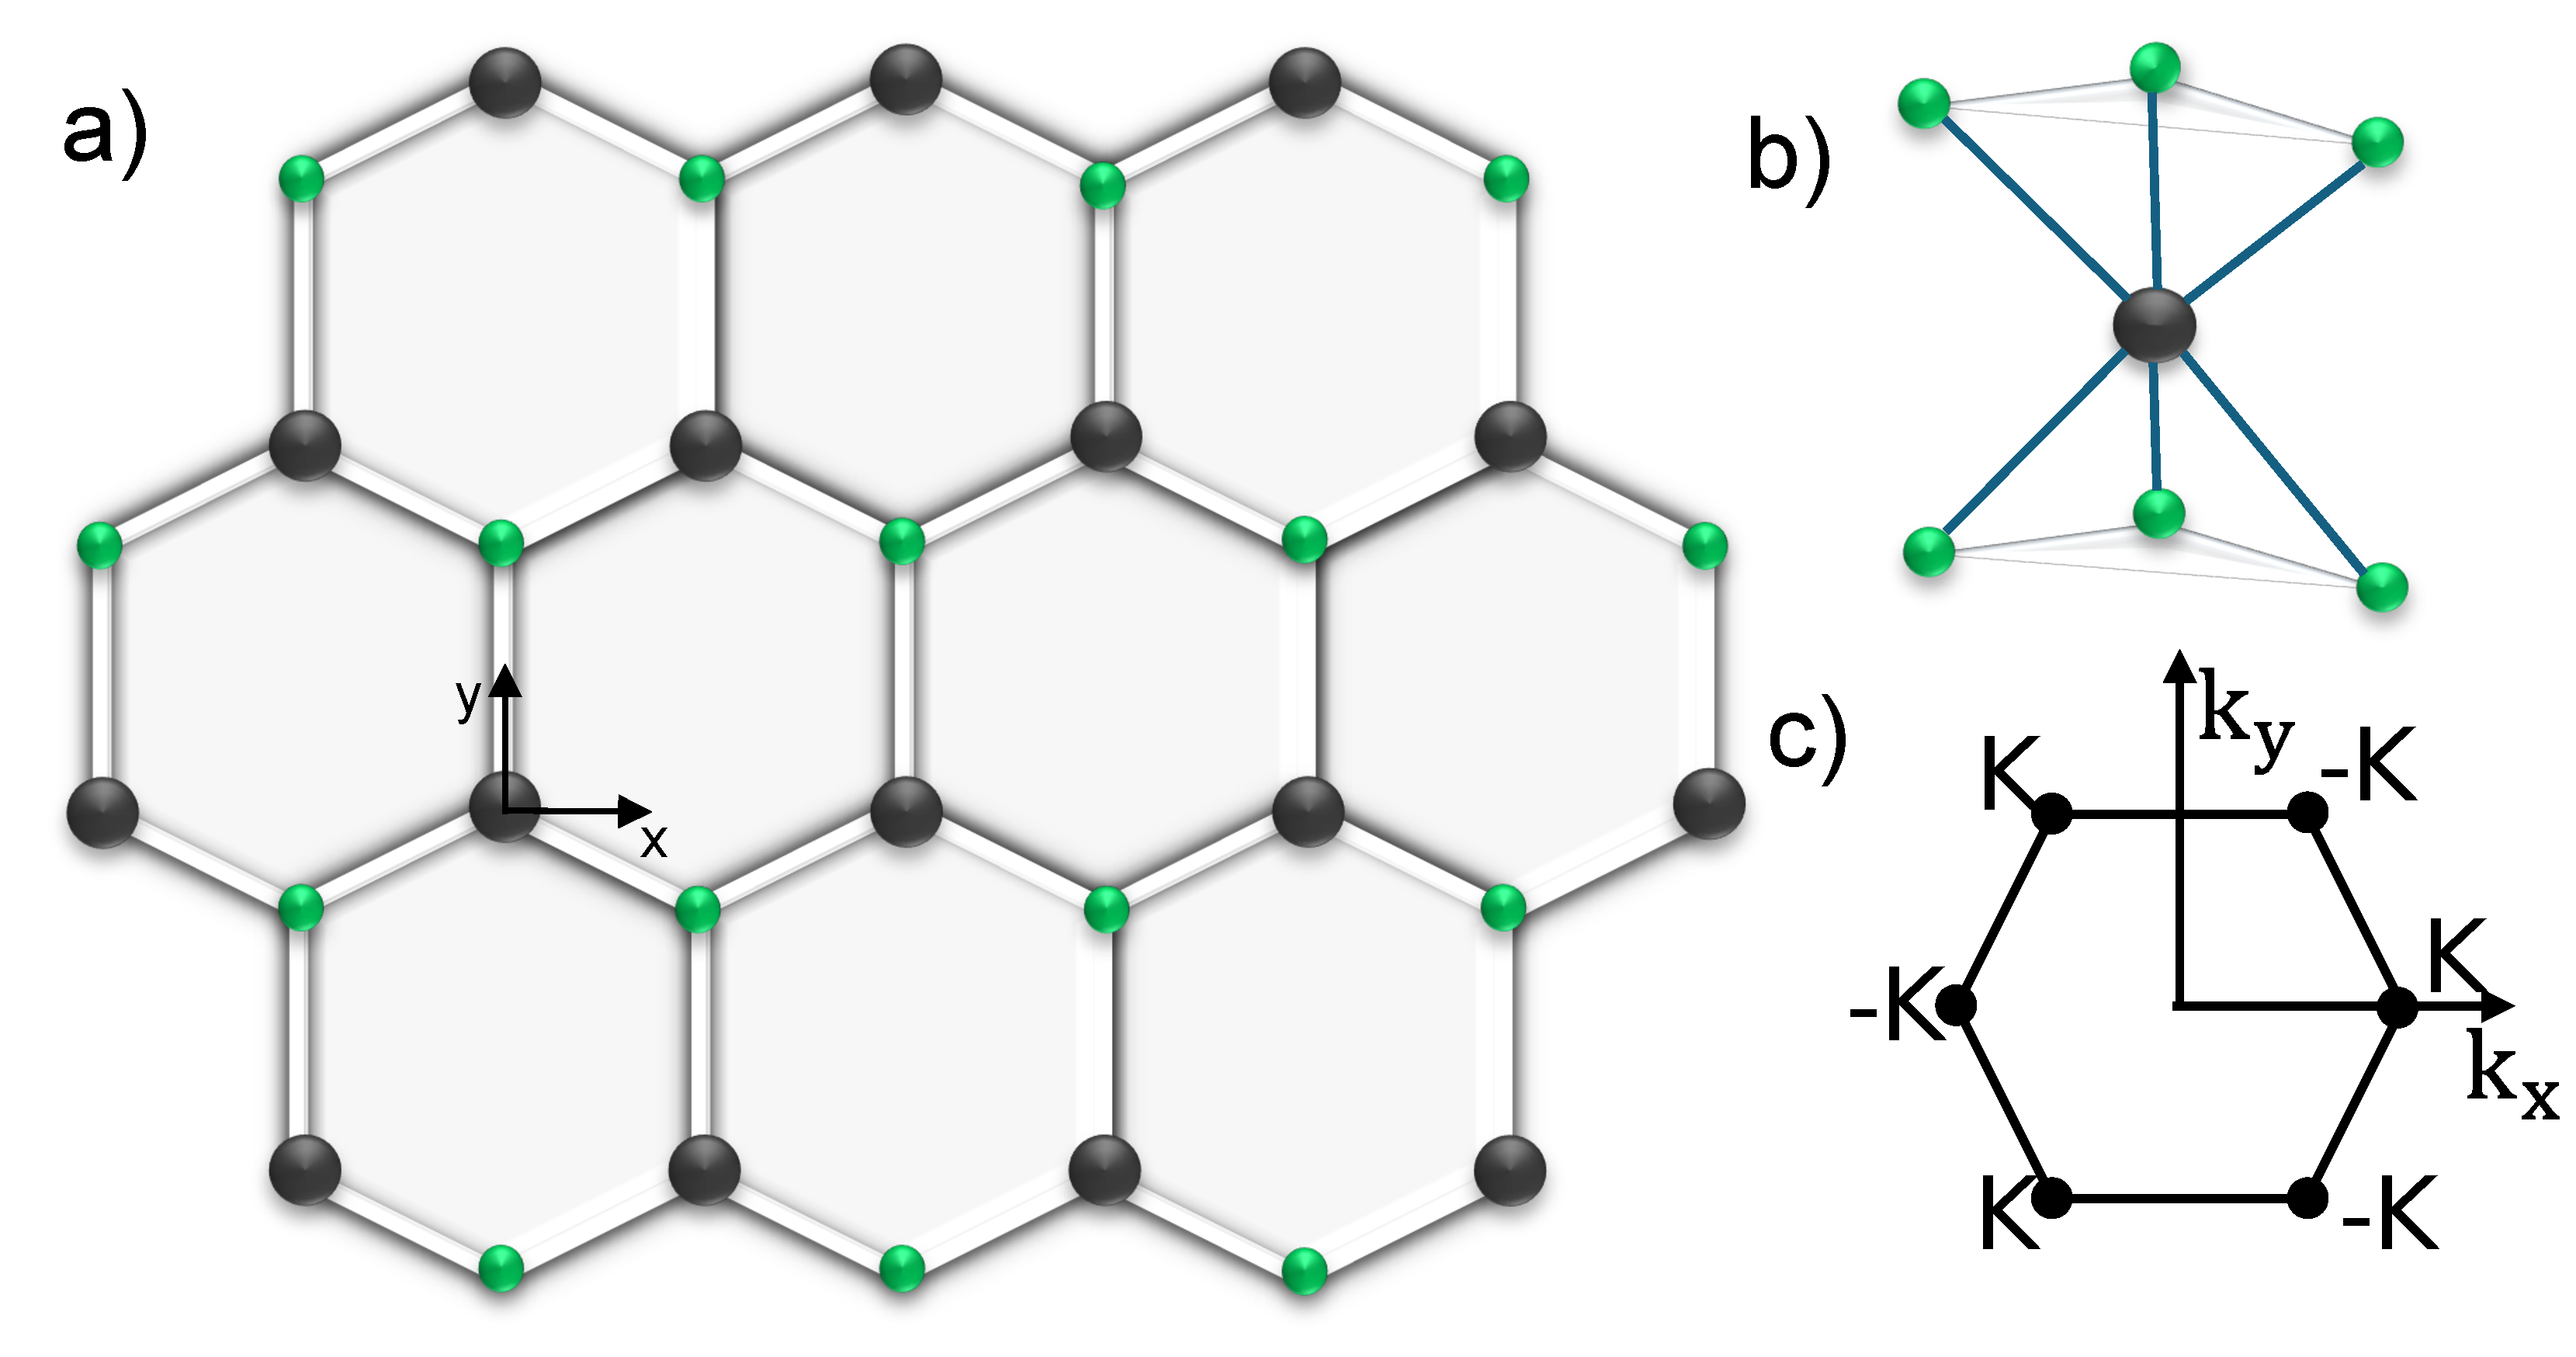
\includegraphics[width=0.75\linewidth]{Images/RS.pdf}
			\caption[TMD structure and its first Brillouin zone]{(a) Top view of monolayer $\mathrm{MX}_2$. The large sphere is \textbf{M} atom and the small sphere is X atom. (b) sideview of monolayer $\mathrm{MX}_2$. (c) The first Brillouin zone and high symmetry points in two dimensional k-space.}
			\label{real space}
		\end{center}
	\end{figure}
	\subsection{Three Band Tight-Binding Model}
\quad In previous ab initio calculations\cite{xiao_coupled_2012,mattheiss_band_1973,lebegue_electronic_2009,zhu_giant_2011,ataca_stable_2012}, Xiao et al. discovered that the monolayer of $MX_2$ with $D_{3h}$ point-group symmetry has a structure as shown in Fig. \ref{real space}. They found that the Bloch states of the monolayer $MoS_2$ near the band edges are primarily composed of $Mo-d$ orbitals, particularly the $d_{z^2}$, $d_{xy}$, and $d_{x^2-y^2}$ orbitals. To accurately capture the band-edge properties in the $K$ and $K'$ valleys, they developed an approximate model for group VII-B TMD consisting of only these three bands and neglecting $X-p$ orbitals, and then extended it to fit the entire Brillouin Zone\cite{liu_three-band_2013}. Denote three M-d bands as:
	\begin{equation}
		\ket{\phi_{1}} = d_{z^2},\quad \ket{\phi_2} = d_{xy}, \quad \ket{\phi_3} = d_{x^2- y^2}.
	\end{equation}
\quad As discussed above, the Bloch states near the band edges mostly consist of Mo-d orbital, therefore we ignore the $\textbf{r}_c$ and the sum over it in hopping energy (\ref{hopping energies}). Each pair of difference basis is assumed to be orthogonal; therefore the overlapping matrix element become:
$$S_{\alpha, \alpha'}(\textbf{k}) = \delta_{\alpha \alpha'}.$$
\quad The hopping energies eq.(\ref{hopping energies}) between the atomic orbitals $\ket{\phi_{\mu}}$ at 0 and $\ket{\phi_{\mu'}}$ at lattice vector $\textbf{R}$ can be obtained as: $$H_{\mu \mu'}(\textbf{k}) =\sum_{\textbf{R}} e^{i\textbf{k}.\textbf{R}}  \bra{\phi_{\mu}(\textbf{r})}  \hat{H} \ket{\phi_{\mu'}(\textbf{r}-\textbf{R})}.$$
\quad Confined by the symmetry of the system, Tight-binding Hamiltonian have the form:
	\begin{equation}
		H^{TNN}(\textbf{k}) =
		\begin{pmatrix}
			V_0  & V_1   & V_2 \\
			V_1^*& V_{11}& V_{12} \\
			V_2^*& V_{12}^* & V_{22} \\
		\end{pmatrix},
	\end{equation}
where
	\begin{align*}
		V_0 &= \varepsilon_1 + 2t_0 (2\cos\alpha\cos\beta + \cos2\alpha) + 2r_0 (2\cos3\alpha\cos\beta+\cos2\beta),\\
		\Re[V_1]&= -2\sqrt{3}t_2 \sin \alpha \sin \beta + 2(r_1 + r_2)\sin 3 \alpha \sin \beta - 2\sqrt{3} u_2 \sin 2\alpha \sin 2\beta,\\
		\Im[V_1] &= 2 t_1 \sin \alpha (2 \cos \alpha +\cos \beta) + 2(r_1 - r_2) \sin 3\alpha \cos \beta + 2u_1 \sin 2\alpha (2\cos 2\alpha + \cos 2\beta)\\
		\Re[V_2] &= 2t_2 (\cos 2\alpha - \cos \alpha \cos \beta) -\frac{2}{\sqrt{3}} (r_1 + r_2 ) (\cos 3\alpha \cos \beta - \cos 2 \beta) + 2u_2 (\cos 4\alpha -\cos 2\alpha \cos 2\beta),\\
		\Im[V_2] &= 2\sqrt{3} t_1 \cos \alpha \sin \beta +\frac{2}{\sqrt{3}} \sin \beta (r_1 -r_2 )(\cos 3\alpha + 2\cos \beta),\\
		V_{11} & = \varepsilon_2 + (t_{11}+3t_{22})\cos \alpha \cos \beta + 2 t_{11} \cos 2\alpha + 4r_{11} \cos 3\alpha \cos \beta \\ &\quad +2 (r_{11} + \sqrt{3} r_{12}) \cos 2\beta + (u_{11} + 3 u_{22})\cos 2 \alpha \cos 2\beta + 2 u_{11} \cos 4\alpha,\\
		\Re(V_{12}) &= \sqrt{3} (t_{22} - t_{11}) \sin \alpha \sin \beta +4 r_{12} \sin 3\alpha \sin \beta + \sqrt{3} (u_{22} - u_{11}) \sin 2\alpha \sin 2\beta,\\
		\Im[V_{12}] &= 4 t_{12} \sin \alpha (\cos \alpha -\cos \beta) + 4u_{12} \sin 2\alpha (\cos 2\alpha - \cos 2\beta),\\
		V_{22} &= \varepsilon_2 +(3t_{11} + t_{22}) \cos \alpha \cos \beta + 2 t_{22} \cos 2 \alpha + 2 r_{11}(2\cos 3\alpha \cos \beta + \cos 2 \beta) \\&\quad + \frac{2}{\sqrt{3}} r_{12} (4\cos 3\alpha \cos \beta - \cos 2\beta) + (3 u_{11} + u_{22}) \cos 2\alpha \cos 2\beta + 2u_{22} \cos 4\alpha,\\
		\text{and}&
		\end{align*}
		\begin{equation}		
			(\alpha,\beta) =  (\frac{1}{2}k_x a, \frac{\sqrt{3}}{2}k_y a),
		\end{equation}
11 additional parameters shown in table \ref{3TB Para} obtained by fitting with FP calculation results. Due to the heavy transition-metal atom M, its spin orbit coupling (SOC) can be large. For simplicity, only the on-site contribution, namely, the $\textbf{L}.\textbf{S}$ term from M atoms, is considered. Using the basis $\{\ket{d_{z^2},\uparrow},\ket{d_{xy},\uparrow},\ket{d_{x^2-y^2,\uparrow}},\ket{d_{z^2},\downarrow},\ket{d_{xy},\downarrow},\ket{d_{x^2-y^2,\downarrow}}\}$, the contribution of SOC to the Hamiltonian can be written as
	\begin{equation}
		H' = \lambda \textbf{L}.\textbf{S}=\frac{\lambda}{2}\begin{pmatrix}
			L_z &0\\
			0 & -L_z
		\end{pmatrix}.
	\end{equation}
\quad In which,
	\begin{equation}
		L_z = \begin{pmatrix}
			0 & 0 & 0\\
			0 & 0 & 2i\\
			0 & -2i& 0
		\end{pmatrix},
	\end{equation}
is the matrix of $\hat{L}_z$ (z component of the orbital angular momentum) in basis of $d_{z^2}, d_{xy}$ and $d_{x^2-y^2}$, and $\lambda$ is characterized for the strength of the SOC. Under these basis, the matrix elements of $\hat{L}_x$ and $\hat{L}_y$ are all zeros. Therefore the Hamiltonian with SOC have the form:
	\begin{equation}
		H(\textbf{k}) = H_{SOC} (\textbf{k}) = I_2 \otimes H^{TNN} (\textbf{k}) +H' = \begin{bmatrix}
			H (\textbf{k}) + \frac{\lambda}{2} L_z & 0\\
			0& H_0 (\textbf{k}) - \frac{\lambda}{2} L_z
		\end{bmatrix}.
	\end{equation}
\quad By finding eigenvalue of Hamiltonian $H$ in each \textbf{k} point on entire BZ, the bands structure will be obtained. The bands structure with the huge bands split at the K and K' point of $\mathrm{MoS}_2$ is caused by SOC is shown in fig.\ref{BS}.
\begin{table}[]
	\begin{center}
		\begin{tabular}{c c c c c c c c c c c c c} 
			\hline
			\hline
				$\varepsilon_1$&$\varepsilon_2$&$t_0$&$t_1$&$t_2$&$t_{11}$&$t_{12}$&$t_{22}$&$r_0$&$r_{1}$&\\
				$r_2$&$r_{11}$&$r_{12}$&$u_{0}$&$u_{1}$& $u_{2}$&$u_{11}$&$u_{12}$&$u_{22}$&$\lambda$\\
				\hline
				%\multicolumn{10}{c}{GGA}                                                      \\
				%$0.683$ & $1.707$ & $-0.146$ & $-0.114$ & $0.506$ & $0.085$ & $0.162$ & $0.073$  & $0.060$ & $-0.236$ \\ $0.067$ & $0.016$ & $0.087$ & $-0.038$ & $0.046$ & $0.001$ & $0.266$ & $-0.176$ & $-0.150$ & $0.073$\\
				%\multicolumn{10}{c}{LDA}                                                      \\
				$0.820$ & $1.931$ & $-0.176$ & $-0.101$ & $0.531$ & $0.084$ & $0.169$ & $0.070$ & $0.070$ & $-0.252$ \\ $0.084$ & $0.019$ & $0.093$ & $-0.043$ & $0.047$ & $0.005$ & $0.304$ & $-0.192$ & $-0.162$ &$0.073$  \\
				\hline
				\hline 
		\end{tabular}
	\caption[Fitting parameters in three-band tight-binding model for $MoS_2$]{Fitting parameters in three-band tight-binding model for local-density approximation (LDA) cases for $MoS_2$.\cite{liu_three-band_2013}}
		\label{3TB Para}
	\end{center}
\end{table}
	\begin{figure}
		\begin{center}
			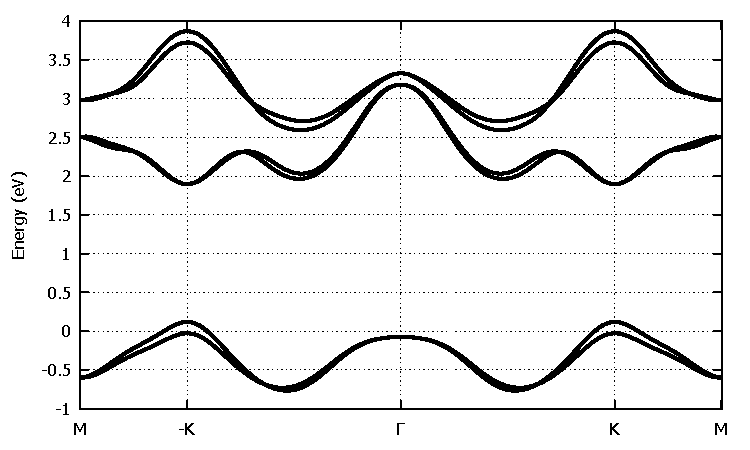
\includegraphics[width= 0.8\linewidth]{Images/BS.pdf}
\caption[Band structure of $\mathrm{MoS}_2$ material along $M\to -\mathrm{K} \to \Gamma \to \mathrm{K}\to M$ direction]{Band structure of monolayer-$\mathrm{MoS}_2$ along $M\to -\mathrm{K} \to \Gamma \to \mathrm{K}\to M$ direction, SOC causes huge splits in band-structure at $\mathrm{K}$ and $-\mathrm{K}$ points.}
			\label{BS}
		\end{center}
	\end{figure}
 	\newpage
	\subsection{System Hamiltonian}
	\subsubsection{First Quantization Hamiltonian}
\quad For the accounting the Coulomb interaction between electron-electron in the many-body system, the system Hamiltonian can be written in form:
	\begin{equation}
		H = H^0 +H^{Coul} = \sum_{i}H_{1e}(\textbf{r}_i) + \frac{1}{2}\sum_{i,j}H^{e-e}(\textbf{r}_i, \textbf{r}_j),
	\end{equation}
where $H_{1e}$ is the single electron Hamiltonian:
	\begin{equation}
		H_{1e}(\textbf{r}_i) = \frac{\textbf{P}^2}{2m} + V_0(\textbf{r}_i).
	\end{equation}
\quad In which the $V_0 (\textbf{r})$ is interaction between electron and ions. The Coulomb interaction between two electrons can be described by:
	\begin{equation}
		\label{H ee}
		H^{e-e}(\textbf{r}_i, \textbf{r}_j) = V_{e-e}(\textbf{r}_i, \textbf{r}_j) = \frac{1}{4\pi \varepsilon \varepsilon_0}\frac{e^2}{|\textbf{r}_i-\textbf{r}_j|},
	\end{equation}
in which the $\varepsilon_0$ is the vacuum permittivity, $\varepsilon$ is relative permittivity. In the present of an external electromagnetic field, the Hamiltonian for an electron in the independent electron approximation takes the form:
	\begin{equation}
		\label{H1e or}
		H_{1e} = \frac{(\textbf{p} + e \textbf{A})^2}{2m} + V_0(\textbf{r}) -e\phi,
	\end{equation}
in which, $\textbf{A}(\textbf{r},t)$ is vector potential and $\phi(\textbf{r},t)$ is scalar potential. With $\textbf{p} = - i\hbar\nabla$, we expand $(\textbf{p}+e\textbf{A})^2 = \textbf{p}^2 + 2e\textbf{A}\textbf{p} + ei \hbar \nabla(\textbf{A}) + (e\textbf{A})^2$. We have $\nabla.(\textbf{A}) = 0$ due to Coulomb gauge, so the Eq. (\ref{H1e or}) becomes
	\begin{equation}
		\label{expand H1e}
		H_{1e} = H^0_{1e} + \frac{e}{m} \textbf{A}.\textbf{p} + \frac{e^2 \textbf{A}^2}{2m} - e\phi,
	\end{equation}
where the $H^0_{1e}$ is stationary Hamiltonian of a single electron particle:
	\begin{equation}
		\label{H01e}
		H^0_{1e} = \frac{\textbf{p}^2}{2m} +V_0 (\textbf{r}),
	\end{equation}
the rest in Eq. (\ref{expand H1e}) shall be defined as the light-matter interaction Hamiltonian $H^{e-L}_{1e}$:
	\begin{equation}
		\label{org LMIH}
		H^{e-L}_{1e} =\frac{e}{m} \textbf{A}.\textbf{p} - e\phi + \frac{e^2 A^2}{2m}.
	\end{equation}
\quad When we choose gauge $\phi = 0$, the electromagnetic field's potential relation between $\textbf{A}$ and $\phi$ becomes:
	\begin{equation}
		\textbf{E} = - \nabla \phi - \pdv{\textbf{A}}{t} = - \pdv{\textbf{A}}{t},
	\end{equation}
	\begin{equation}
		\textbf{A}(\textbf{r},t) = -\int_{-\infty}^t dt' \textbf{E}(\textbf{r}, t'). 
	\end{equation}
\quad Substituting $\phi = 0$ into Eq. (\ref{expand H1e}),
	\begin{equation}
		H^{VG}_{1e}= H^0_{1e} + \frac{e}{m}\textbf{A}.\textbf{p} + \frac{e^2\textbf{A}^2}{2m}.
	\end{equation}
\quad From the definition of the velocity operator $\textbf{v}= \frac{i}{\hbar} [H_{1e}, \textbf{r}] = \frac{\textbf{p}+e\textbf{A}}{m}$, $H^{VG}_{1e}$ can be written in the form
	\begin{equation}
		\label{H VG}
		H^{VG}_{1e} = H^0_{1e} + e \textbf{A}.\textbf{v} - \frac{e^2A^2}{2m}.
	\end{equation}
\quad In velocity gauge, the light-matter interaction Hamiltonian (\ref{org LMIH}) have the form:
	\begin{equation}
		\label{e-L Hamiltonian}
		H^{e-L}_{1e} =\frac{e}{m} \textbf{A}.\textbf{p} + \frac{e^2 A^2}{2m}.
	\end{equation}
\quad Combining Eqs. (\ref{H01e}), (\ref{H ee}), and (\ref{e-L Hamiltonian}), we obtain the many-body Hamiltonian describing the system of electrons interacting with an external electromagnetic field:
	\begin{equation}
		\label{1st Quanti}
		H =  \sum_{i} H^0_{1e} (\textbf{r}_i) + \sum_{i} H^{e-L}_{1e} (\textbf{r}_i,t) + \frac{1}{2} \sum_{\textbf{r}_i, \textbf{r}_j}H^{e-e}(\textbf{r}_i, \textbf{r}_j).
	\end{equation}
	\subsubsection{Second Quantization Hamiltonian}
\quad From Eq. (\ref{1st Quanti}), the second quantization Hamiltonian in Bloch basis $\{\ket{\psi_{\lambda \textbf{k}}}\}$ has the form:
	\begin{align}
		\hat{H} &= \hat{H}^0 + \hat{H}^{e-L}  + \hat{H}^{e-e}\nonumber,\\
		\label{Second Hamiltonian}
		\hat{H}^0 &= \sum_{\lambda \lambda' \textbf{k}\textbf{k}'} \bra{\psi_{\lambda \textbf{k}}} H^0_{1e} (\textbf{r})\ket{\psi_{\lambda' \textbf{k}'}} c^\dg_{\lambda \textbf{k}} c_{\lambda' \textbf{k}
		'} ,\\
		\hat{H}^{e-L} &= \sum_{\lambda \lambda' \textbf{k}\textbf{k}'} \bra{\psi_{\lambda \textbf{k}}} H^{e-L} (\textbf{r})\ket{\psi_{\lambda' \textbf{k}'}} c^\dg_{\lambda \textbf{k}} c_{\lambda' \textbf{k}
			'}\nonumber ,\\
\hat{H}^{e-e}	&= \frac{1}{2} \sum_{\textbf{k}, \textbf{k}', \textbf{q}} \sum_{\alpha \beta \gamma \delta} \bra{\psi_{\alpha \textbf{k + q}} \psi_{\beta \textbf{k}' - \textbf{q}}} V_{e-e} \ket{\psi_{\gamma \textbf{k}'} \psi_{\delta \textbf{k}}} c_{\alpha, \textbf{k}+\textbf{q}}^\dg c_{\beta, \textbf{k}' - \textbf{q}}^\dg c_{\gamma, \textbf{k}}c_{\delta, \textbf{k'}} \nonumber,
	\end{align}
in which the basis is orthonormal: $\braket{\psi_{\lambda \textbf{k}}}{\psi_{\lambda' \textbf{k}'}} = \delta_{\lambda\lambda'}\delta_{\textbf{k}\textbf{k'}}$, and the creation and annihilation operators satisfy the anti-commutator relations:
	\begin{equation}
		\label{fermion comm}
		\big\{c_{\lambda,\textbf{k}}, c_{\lambda', \textbf{k}'}\big\} =\big\{c^\dg_{\lambda,\textbf{k}}, c^\dg_{\lambda', \textbf{k}'}\big\} = 0, \quad \big\{c_{\lambda,\textbf{k}}, c^\dg_{\lambda', \textbf{k}'}\big\} = \delta_{\lambda,\lambda'}\delta_{\textbf{k},\textbf{k'}}.
	\end{equation}
\quad If we choose the basis is a set of eigenvectors of $H^0_{1e}$ then $H^0$ becomes:
	\begin{equation}
		\hat{H}^0 = \sum_{\lambda \textbf{k}} \varepsilon_{\lambda}(\textbf{k})c^\dg_{\lambda \textbf{k}} c_{\lambda \textbf{k}}.
	\end{equation}
\quad It is worth noting that the eigenvector of $H^0_{1e}$ does not satisfy the orthonormality in general but only satisfies it if $\textbf{k} \approx \textbf{k}'$. In VG, the elements of interaction Hamiltonian matrix $\bra{\psi_{\lambda\textbf{k}}}H^{e-L}(\textbf{r},t)\ket{\psi_{\lambda'\textbf{k}'}}$ is:
	\begin{align}
		\bra{\psi_{\lambda\textbf{k}}}H^{e-L}(\textbf{r},t)\ket{\psi_{\lambda'\textbf{k}'}} &= \bra{\psi_{\lambda\textbf{k}}}\frac{e}{m}\textbf{A}(\textbf{r},t).\textbf{p}\ket{\psi_{\lambda'\textbf{k}'}} +\frac{e^2 A^2}{2m} \delta_{\lambda \lambda'}\delta_{\textbf{k}\textbf{k}'} \nonumber\\
		&\approx \frac{e}{m}\textbf{A}(t). \bra{\psi_{\lambda\textbf{k}}}\textbf{p}\ket{\psi_{\lambda'\textbf{k}'}} + \frac{e^2 A^2}{2m} \delta_{\lambda \lambda'}\delta_{\textbf{k}\textbf{k}'},
	\end{align}
where
	\begin{align}
		\bra{\psi_{\lambda\textbf{k}}}\textbf{p}\ket{\psi_{\lambda'\textbf{k}'}} &= \int \frac{d^3 r}{V} e^{-i\textbf{k}.\textbf{r}}u^{*}_{\lambda \textbf{k}}(\textbf{r}) \hat{\textbf{p}}(e^{i\textbf{k}'.\textbf{r}} u_{\lambda'\textbf{k}'}(\textbf{r})) \nonumber \\
		& =	\int \frac{d^3 r}{V} e^{i(\textbf{k}'-\textbf{k}).\textbf{r}}u^{*}_{\lambda \textbf{k}}(\textbf{r}) (\hbar \textbf{k}+\hat{\textbf{p}}) u_{\lambda'\textbf{k}'}(\textbf{r}) \nonumber \\
		\label{p before wave approximate}
		& = \frac{1}{N} \sum_{i}^{N} e^{i(\textbf{k}'-\textbf{k})\textbf{R}_i} \int_{V_{Cell}} \frac{d^3r}{V_{Cell}}e^{i(\textbf{k}'-\textbf{k}).\textbf{r}}u^{*}_{\lambda \textbf{k}}(\textbf{r}) (\hbar \textbf{k}+\hat{\textbf{p}}) u_{\lambda'\textbf{k}'}(\textbf{r}).
	\end{align}
\quad We include the Long-wavelength approximation $\textbf{k}',\textbf{k} << \frac{2\pi}{a}$ to have:
	\begin{align}
		\bra{\psi_{\lambda\textbf{k}}}\textbf{p}\ket{\psi_{\lambda'\textbf{k}'}} &\approx \frac{1}{N} \sum_{i}^{N} e^{i(\textbf{k}'-\textbf{k})\textbf{R}_i} \int_{V_{Cell}} \frac{d^3r}{V_{Cell}}u^{*}_{\lambda \textbf{k}}(\textbf{r}) (\hbar \textbf{k}'+\hat{\textbf{p}}) u_{\lambda'\textbf{k}'}(\textbf{r})\nonumber \\
		& \approx \frac{1}{N} \sum_{i}^{N} e^{i(\textbf{k}'-\textbf{k})\textbf{R}_i} (\hbar \textbf{k}' \bra{u_\lambda \textbf{k}} \ket{u_{\lambda'}\textbf{k}'} + \bra{u_\lambda \textbf{k}} \hat{\textbf{p}}\ket{u_{\lambda'}\textbf{k}'}),
		\label{on going}
	\end{align}
	\quad using relation $
\sum_{i}^{N} e^{(\textbf{k}'-\textbf{k})\textbf{R}_i}= N\delta_{\textbf{k'},\textbf{k}}$. Eq. (\ref{on going}) becomes
	\begin{equation}
		\label{p after LWA}
		\quad \bra{\psi_{\lambda\textbf{k}}}\textbf{p}\ket{\psi_{\lambda'\textbf{k}'}} \approx (\textbf{p}_{\lambda\lambda'}(\textbf{k}) + \hbar \textbf{k} \delta_{\lambda\lambda'}) \delta_{\textbf{k}, \textbf{k}'}.
	\end{equation}
\quad In which,
	\begin{equation}
		\textbf{p}_{\lambda\lambda'}(\textbf{k}) = \bra{u_{\lambda\textbf{k}}}\textbf{p}\ket{u_{\lambda'\textbf{k}}}.
	\end{equation}
\quad It depends on whether the momentum matrix elements \(\textbf{p}_{\lambda\lambda'}(\textbf{k})\) are equal to 0 or not, to determine whether the transition between \(\lambda\) and \(\lambda'\) at $\textbf{k}$ is allowed. Using $H^0_{1e}(\textbf{k})= e^{-i\textbf{k}\textbf{r}} H^{0}_{1e} e^{i\textbf{k}\textbf{r}}$ and the relation: $[H^0_{1e},\textbf{r}] = -i\frac{\hbar}{m}\textbf{p}$ to have
	\begin{equation}
		\label{momentum}
		\textbf{p}_{\lambda\lambda'}(\textbf{k}) = \frac{m}{\hbar} \bra{u_{\lambda \textbf{k}}} \nabla_{\textbf{k}}H^0_{1e}(\textbf{k}) \ket{u_{\lambda'\textbf{k}}}.
	\end{equation}
\quad Eq. (\ref{momentum}) enables us to numerically calculate the momentum matrix elements at discrete k-points. Therefore, the light-matter interaction part of the second quantization Hamiltonian takes the following form:
	\begin{equation}
		\hat{H}^{e-L} = \frac{e}{m}\textbf{A}(t)\vdot\sum_{\lambda\lambda' \textbf{k}}\textbf{p}_{\lambda \lambda'}(\textbf{k})c^\dg_{\lambda\textbf{k}}c_{\lambda' \textbf{k}} + \bigg(\hbar \textbf{k} + \frac{e^2 \textbf{A}^2}{2m}\bigg)\sum_{\lambda \textbf{k}} c^\dg_{\lambda \textbf{k}} c_{\lambda\textbf{k}}.
	\end{equation}
\quad The $H^{e-e}$ derivation is presented in Appendix \ref{V ee derivation}. Thus, the many-body  Hamiltonian in second quantization in VG has the form:
		\begin{align}
		\label{H with Coulomb in second}
		\hat{H} =& \hat{H}^0_{1e} +\hat{H}^{e-e} + \hat{H}^{e-L} \nonumber \\
		=&  \sum_{\lambda\textbf{k}} \varepsilon_\textbf{k} c_{\lambda\textbf{k}}^\dg c_{\lambda\textbf{k}} \nonumber \\ 
		&+ \frac{1}{2} \sum_{\textbf{k}, \textbf{k}', \textbf{q}} \sum_{\alpha \beta \gamma \delta} W^{\alpha \beta \gamma \delta}_{\textbf{k},\textbf{k'},\textbf{q}} c_{\alpha, \textbf{k}+\textbf{q}}^\dg c_{\beta, \textbf{k}' - \textbf{q}}^\dg c_{\gamma, \textbf{k}}c_{\delta, \textbf{k'}} \nonumber \\
		&+ \frac{e}{m}\textbf{A}(t)\vdot\sum_{\lambda\lambda' \textbf{k}}\textbf{p}_{\lambda \lambda'}(\textbf{k})c^\dg_{\lambda\textbf{k}}c_{\lambda' \textbf{k}} + \bigg(\hbar \textbf{k} + \frac{e^2 \textbf{A}^2}{2m}\bigg)\sum_{\lambda \textbf{k}} c^\dg_{\lambda \textbf{k}} c_{\lambda\textbf{k}},
	\end{align}
\quad where the Coulomb interaction matrix elements are:
	\begin{equation}
		W^{\alpha \beta \gamma \delta}_{\textbf{k}, \textbf{k}',\textbf{q}} = V_{e-e}(\textbf{q}) \braket{u_{\alpha\textbf{k} +\textbf{q}}}{u_{\delta\textbf{k}}} \braket{u_{\beta\textbf{k}' -\textbf{q}}}{u_{\gamma \textbf{k}'}},
	\end{equation}
\quad with the 2-D Coulomb interaction in momentum space:
	\begin{equation}
		\label{2D coulomb}
		V_{e-e}(\textbf{q}) = \frac{e^2}{2\varepsilon\varepsilon_0 L^2} \frac{1}{|\textbf{q}|}.
	\end{equation}
	\subsection{Semiconductor Bloch Equation}
\quad With definition of density matrix elements,
	\begin{equation}
		\rho_{\lambda \lambda'}(\textbf{k}) = \ev{c^\dg_{\lambda'\textbf{k}} c_{\lambda\textbf{k}}},
	\end{equation}
\quad We use the equation of motion in Heisenberg picture for operator $c^\dg_{\lambda'\textbf{k}} c_{\lambda\textbf{k}}$ and take its expectation value to have:
	\begin{equation}
		\label{Heisenberg eq}
		\dv{}{t}\ev{c^\dg_{\lambda'\textbf{k}} c_{\lambda\textbf{k}}} = \frac{i}{\hbar}\ev{\big[H,c^\dg_{\lambda'\textbf{k}} c_{\lambda\textbf{k}} \big]}.
	\end{equation}
\quad Through the derivation in Appendix \ref{Motion Equation}, we have obtained the Semiconductor Bloch Equation(s) with Coulomb interaction in the Hartree-Fock approximation:
\begin{align}
	\label{SBE HF}
\dv{ }{t}\rho_{\lambda\lambda'}(\textbf{k}) =& - \frac{i}{\hbar} (\varepsilon_\lambda(\textbf{k}) - \varepsilon_{\lambda'} (\textbf{k}))\rho_{\lambda \lambda'}(\textbf{k}) - \frac{ie}{\hbar m} \textbf{A}(t)\sum_{\mu}\left[\textbf{p}_{\lambda\mu}(\textbf{k})\rho_{\mu \lambda'}(\textbf{k}) - \rho_{\lambda\mu}(\textbf{k})\textbf{p}_{\mu \lambda'}(\textbf{k})\right] \nonumber \\
&+ \frac{i}{\hbar}\left[\Omega_{\lambda \mu}(\textbf{k})\rho_{\mu \lambda'}(\textbf{k}) - \rho_{\lambda\mu}(\textbf{k}) \Omega_{\mu \lambda'} (\textbf{k})\right] +\dv{ }{t}\rho_{\lambda\lambda'}(\textbf{k})\bigg|_{\mathrm{scat.}},
\end{align}
\quad where
\begin{equation}
\Omega_{\mu\nu} (\textbf{k})=\sum_{\alpha \beta \textbf{q}} W^{\alpha \mu \beta \nu}_{\textbf{k},\textbf{k}+\textbf{q},\textbf{q}} \rho_{\alpha\beta} (\textbf{k}+\textbf{q}).
\end{equation}
\quad The term "interband polarization" describes the decay of quantum coherence. A common and generally accurate approximation is to use the dephasing time parameter $T_2$, also known as the transverse relaxation time. This simple approximation is limited by nonlinear and non-Markovian effects, which can be ignored in this work. Therefore,
\begin{equation}
	\label{off diag scat.}
	\bigg(\dv{ }{t} \rho(\textbf{k})\bigg|_{\mathrm{scat.}}\bigg)_{\lambda \lambda'} \approx -\frac{\rho_{\lambda \lambda'}(\textbf{k})}{T_2}\quad \forall \lambda \neq \lambda'. 
\end{equation}
Including Eq. (\ref{off diag scat.}) into Eq. (\ref{SBE HF}), we obtain the Semiconductor Bloch Equations\cite{haug_quantum_2009}:
\begin{align}
	\label{SBE}
	\dv{ }{t}\rho_{\lambda\lambda'}(\textbf{k}) = &- \frac{i}{\hbar} (\varepsilon_\lambda(\textbf{k}) - \varepsilon_{\lambda'} (\textbf{k}))\rho_{\lambda \lambda'}(\textbf{k}) - \frac{ie}{\hbar m} \textbf{A}(t)\sum_{\mu}(\textbf{p}_{\lambda\mu}(\textbf{k})\rho_{\mu \lambda'}(\textbf{k}) - \rho_{\lambda\mu}(\textbf{k})\textbf{p}_{\mu \lambda'}(\textbf{k})) \nonumber \\
	&+ \frac{i}{\hbar}(\Omega_{\lambda \mu}(\textbf{k})\rho_{\mu \lambda'}(\textbf{k}) - \rho_{\lambda\mu}(\textbf{k}) \Omega_{\mu \lambda'} (\textbf{k})) -\frac{1}{T_2}\rho_{\lambda\lambda'}(\textbf{k})(1-\delta_{\lambda\lambda'}),
\end{align}
\quad where
\begin{equation}
	\Omega_{\mu\nu} (\textbf{k})=\sum_{\substack{\alpha\beta \textbf{q}}} W^{\alpha \mu \beta \nu}_{\textbf{k},\textbf{k}+\textbf{q},\textbf{q}} \rho_{\alpha\beta} (\textbf{k}+\textbf{q}).
\end{equation}
\subsection{Polarization Density}
\quad Polarization density is calculated from the trace of dipole and density matrix multiplication
\begin{equation}
\label{polar density or}
\textbf{P}(t) = \frac{e}{L^2} \sum_{\textbf{k}}\Tr[\vec{\xi}(\textbf{k})\rho(\textbf{k},t)] = \frac{e}{L^2}\sum_{\substack{\lambda \lambda'\textbf{k}}} \vec{\xi}_{\lambda \lambda' }(\textbf{k})\rho_{\lambda' \lambda}(\textbf{k},t).
\end{equation}
\quad Taking the sum over all $\textbf{k}$-points in the first BZ in 2D \textbf{k}-grid through the integral
\begin{equation}
\sum_{\textbf{k}}... \to \frac{L^2}{(2\pi)^2}\int_{\mathrm{BZ}} d^2 k...
\end{equation}
\quad Including it into polarization density Eq. (\ref{polar density or}) to have:
\begin{equation}
	\label{polar}
\textbf{P}(t) = \frac{e}{L^2} \sum_{\textbf{k}} \Tr[\vec{\xi} (\textbf{k}) \rho(\textbf{k},t)] = \frac{1}{(2\pi)^2} \sum_{\lambda\lambda'}	\int \vec{\xi}_{\lambda \lambda'} (\textbf{k}) \rho_{\lambda'\lambda}(\textbf{k},t)d\textbf{k},
\end{equation}
in which the dipole $\vec{\xi}_{\lambda \lambda'}(\textbf{k})$ can be calculated through $\textbf{p}_{\lambda \lambda'}(\textbf{k})$ (derived in appendix \ref{Dipole Matrix Elements}):
\begin{equation}
	\vec{\xi}_{\lambda \lambda'} (\textbf{k}) = -\frac{i\hbar }{m} \frac{\textbf{p}_{\lambda \lambda'}(\textbf{k})}{\varepsilon_{\lambda}(\textbf{k}) - \varepsilon_{\lambda'}(\textbf{k})}.
\end{equation}
\quad The numerical result of Eq. (\ref{polar}) will be obtained by using the Riemann sum integral.
\newpage
\section{Numerical Methods}
\subsection{Numerical Sum Over k-Space}
\quad Monolayer TMD's actual lattice, denoted as $MX_2$, possesses the $D_3h$ point-group symmetry, which is illustrated in Fig. \ref{real space}. The 2D first Brillouin zone takes on the shape of a hexagon. This study concentrates on the linear abortion spectrum, a feature that relies heavily on the k-point with the direct band gap of this material. To numerical calculate the Eq. (\ref{polar}), we need to take numerical integral over the first BZ, which is inconvenient when working with the hexagon shape. Furthermore, a direct band gap is observed at the K and K' points in the first BZ, as depicted in Fig. (\ref{BS}). There are three K and three K' points situated at the edge of the first BZ as shown in fig. \ref{Rhombus}, with each point being shared between three BZ. Consequently, we need to calculate the average numerical position by adding up the positions and then dividing by the number of points, which can pose further challenges for the many-body problems we are addressing.\\\null
\quad To address this, we introduce the use of the rhombus primitive cell, as shown in Fig. 3. This cell is constructed from 4 M-points located between K and K' on the edge of the hexagon, enabling us to focus on the properties of K and K' points both individually and in pairs.
\begin{figure}[h]
	\begin{center}
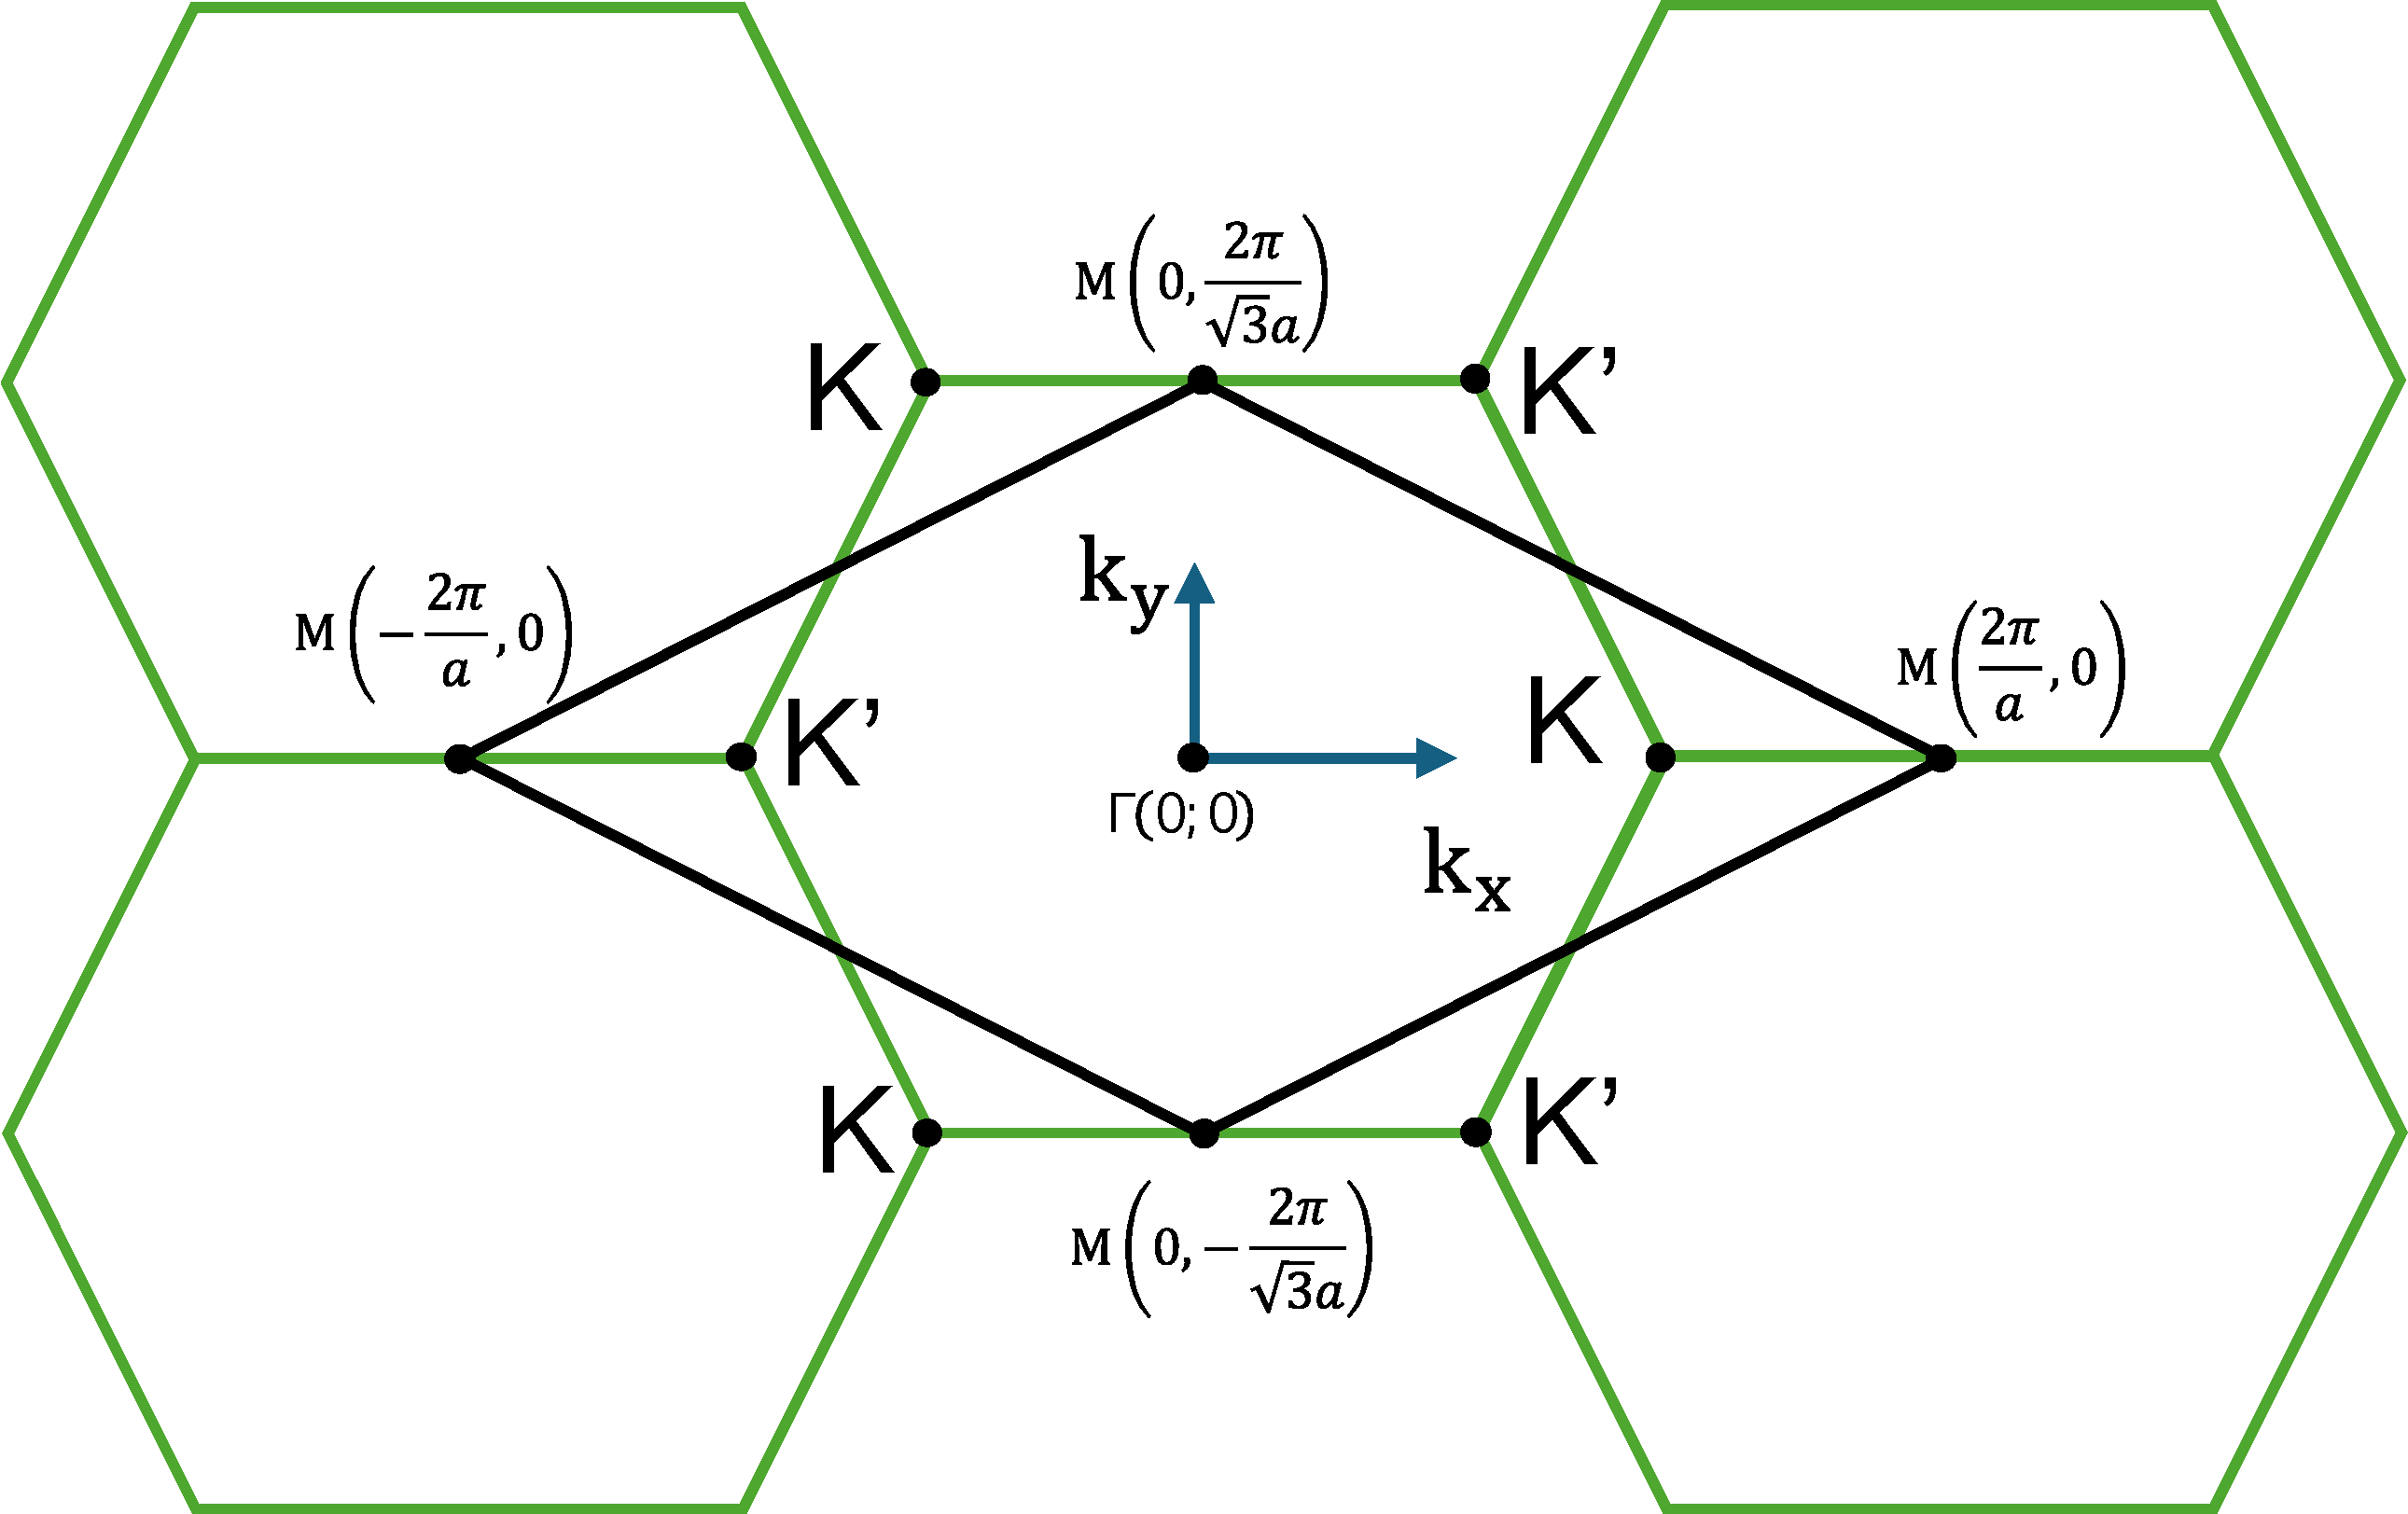
\includegraphics[width= 0.75\linewidth]{Images/Rhombus.pdf}
\caption[Rhombus primitive unit cell in compare with hexagon primitive unit cell (the first Brillouin zone)]{Rhombus primitive unit cell constructed through four M-points, which has the same area as the first Brillouin zone (the green Hexagon with six corners at "K-point" and "K'-point")}
\label{Rhombus}
	\end{center}
\end{figure}\\\null
\quad In order to establish a new coordinate system, we will utilize the two unit vectors located at the left corner of the rhombus $u_1 = (2\pi/3a,2\pi/\sqrt{3}a)$ and $u_2 = (2\pi/3a,-2\pi/\sqrt{3}a)$ as shown in Fig. \ref{rhombuskgrid}, which will be reference to as the "Rhombus basis" hereinafter. Consider a point $\textbf{P}$, which have coordinate $(v_1, v_2)$ in rhombus basis and coordinate $(k_x,k_y)$ in rectangular basis. These coordinate have the relation through the transformation:
\begin{equation}
	\begin{pmatrix} k_x \\ k_y \end{pmatrix}
	= \frac{2\pi}{a} \begin{pmatrix}
		1 & 1\\ \frac{1}{\sqrt{3}} & -\frac{1}{\sqrt{3}}\end{pmatrix} \begin{pmatrix} v_1 \\v_2\end{pmatrix} - \begin{pmatrix} \frac{2\pi}{a} \\ 0\end{pmatrix},\quad  \begin{pmatrix} v_1 \\v_2\end{pmatrix}
		= \frac{a}{4\pi} \begin{pmatrix}
		1 & \sqrt{3}\\1 & -\sqrt{3}\end{pmatrix}\begin{pmatrix} k_x \\ k_y \end{pmatrix}  + \begin{pmatrix} 1/2 \\ 1/2\end{pmatrix}, 
\end{equation}
\quad Since the $v_1,v_2$ is a continuous variable, we need to convert it into discrete coordinates in order to proceed with a numerical solution. To do this, we divide the vectors $u_1$ and $u_2$ into $n$ equal segments, which are then labeled as $n_{1}$ and $n_{2}$, respectively. We discrete the continuous coordinate $(v_1,v_2)$ in term of $(n_{1},n_{2})$:
$$\begin{cases}
v_1 = n_{1} \frac{u_1}{n}\\
v_2 = n_{2} \frac{u_2}{n}
\end{cases}, n_1, n_2 \in \{0,1,..,n\}.$$
\begin{figure}
	\begin{center}
		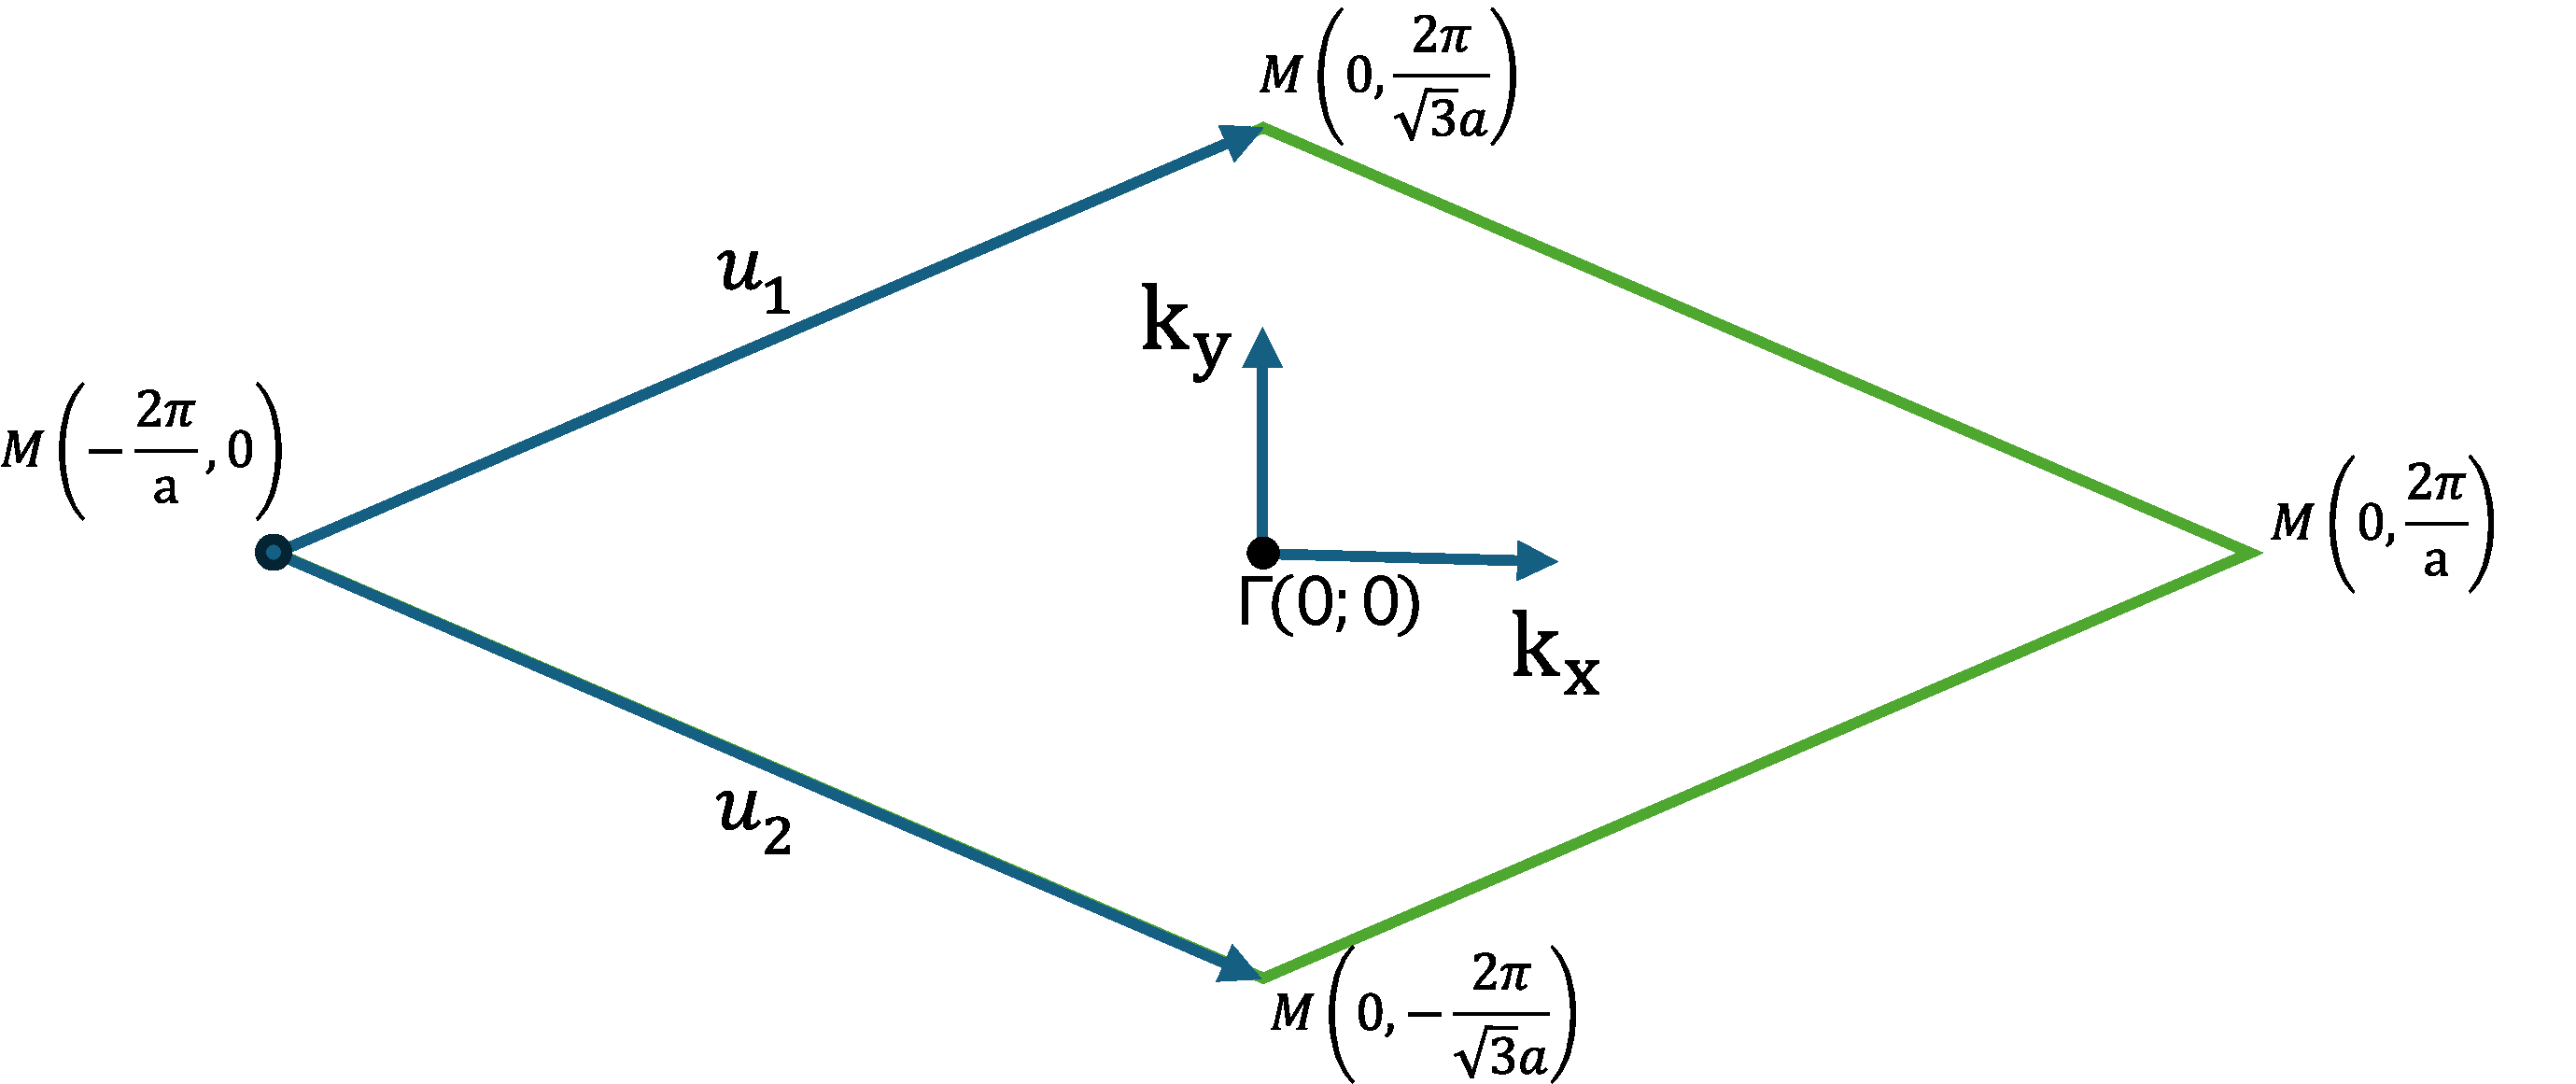
\includegraphics[width=0.5\linewidth]{Images/rhombuskgrid.pdf}
		\caption{New basis Based on the rhombus unit vectors}
		\label{rhombuskgrid}
	\end{center}
\end{figure}
\subsection{Cut-off K-point Technique}
\quad In our research, we are focusing on the transition between the valence and conduction bands around the K and K' points. We achieve this by using a small-intensity electric field and limiting the photon energy to around the band gap energy $E_{gap}$. However, the calculation of the Coulomb interaction for every point in the rhombus with other points all over the rhombus is not efficient in terms of time cost, and convergence. As demonstrated in the 2-D Coulomb interaction Eq. (\ref{2D coulomb}), the Coulomb potential is inversely proportional to the distance between two points in k-space. To address this issue, we are introducing a technique to limit the points taken into account in the Coulomb interaction part.\\\null
\begin{figure}[ht]
	\begin{center}
		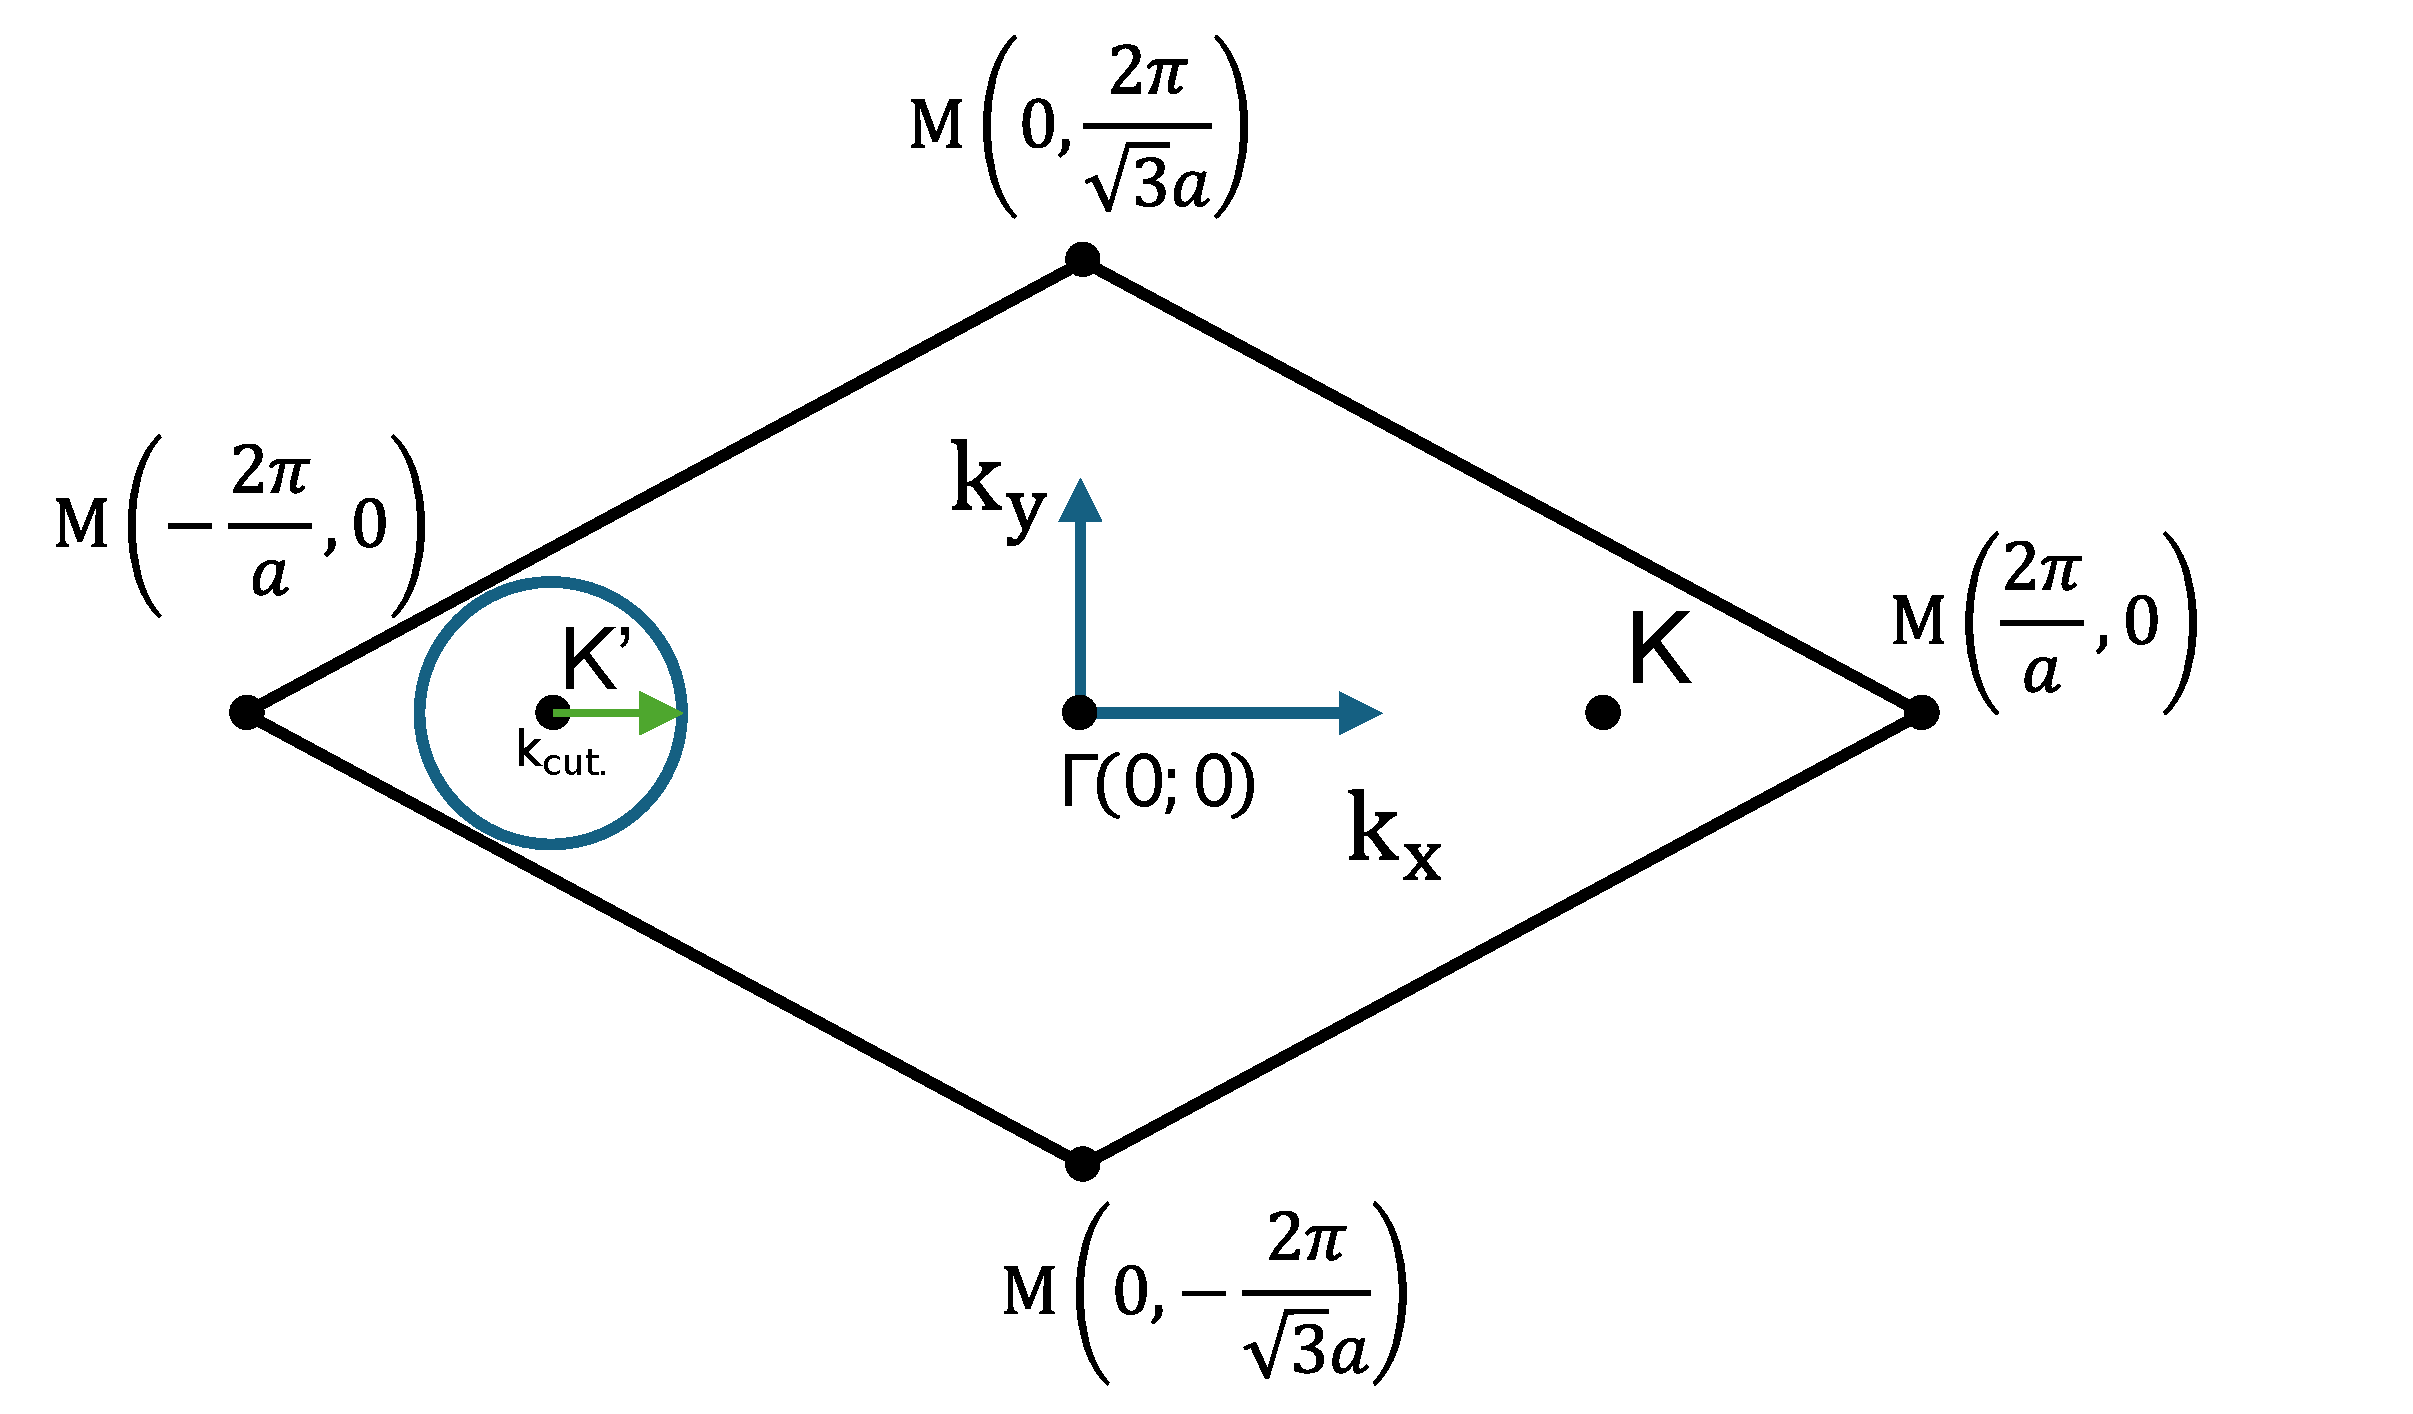
\includegraphics[width = 0.5 \linewidth]{Images/kcutoff.pdf}
		\caption{k-radius show the cutoff circle around K' points}
		\label{k cutoff}
	\end{center}
\end{figure}
\quad In the diagram shown in Fig. \ref{k cutoff}, a circle is drawn around the K' point with a radius of $k_{cut.}$. When calculating the Eq. (\ref{SBE}) at a k-point, if this k-point is outside the circle, we use
$$\Omega_{\mu \nu}(\textbf{k}) = 0 \quad \forall \mu,\nu.$$
\quad When dealing with k-point inside the circle, we only consider interactions with other points inside the circle. This reduces the computational load significantly. In a 2-dimensional system, each doubling of k-points results in a 32-fold increase in simulation time (we calculate on both K and K'). However, by focusing around the K/K' point and reducing the number of k-points, the time cost only increases by approximately 8 to 10 times.\\\null
\quad In summary, we approximate the Coulomb interaction matrix elements:
$$W^{\alpha \mu \beta \nu}_{\textbf{k},\textbf{k}',\textbf{q}} \approx W^{\alpha \mu \beta \nu}_{\textbf{k},\textbf{k}',\textbf{q}} \theta(k_{cut.} - |\textbf{k} - \textbf{k}_{K'}|) \theta(k_{cut.} - |\textbf{k}' - \textbf{k}_{K'}|).$$
\quad Where $\theta(k)$ represents the Heaviside function, the Coulomb interaction is excluded if either point is outside the circle. The same process applies for the K point.
\subsection{Absorption and Electromagnetic Field}
\quad The linear absorption spectrum is determined by\cite{haug_quantum_2009}
\begin{equation}
	\alpha(\omega) \propto \Im{\frac{P(\omega)}{E(\omega)}}.
	\label{absorpt}
\end{equation}
\quad In which $\textbf{P}(\omega)= \int_{-\infty}^{\infty}\textbf{P}(t) e^{i\omega t} dt$ and $\textbf{E}(\omega) = \int_{-\infty}^{\infty}\textbf{E}(t) e^{i\omega t} dt$ are the Fourier transform for polarization density and electric field. These integral can be approximated using a Riemann sum with the cut-off point by using condition $\textbf{E}(t_{cutoff}) \lessapprox 10^{-6} \abs{\max{\textbf{E}(t)}}$ and $\textbf{P}(t_{cutoff}) \lessapprox 10^{-6} \abs{\max{\textbf{P}(t)}}$. In this work, we are using the electric field in form:
\begin{equation}
	\textbf{E}(t) = E_0 e^{-\frac{t^2}{\tau_L^2}}(cos(\omega_0t), 0),
\end{equation} 
with the $E_0$ is the maximal amplitude, $\hbar\omega_0 = E_{\mathrm{gap}}$, $\tau_L$ is the duration of the Gaussian envelope, and $t$ is time, all will be calculated in SI units. The $E_x(t)$ and its Fourier transform shape are shown in Fig. \ref{Et}.\\
\begin{figure}
	\begin{center}
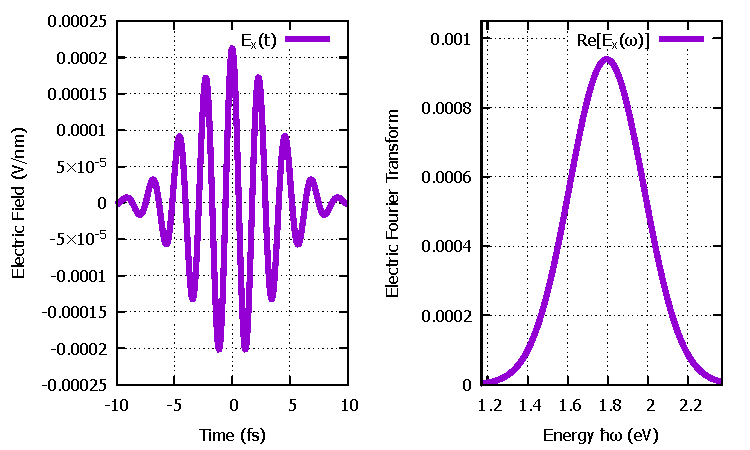
\includegraphics[width = 0.75\linewidth]{Images/EAt.pdf}
\caption{Electric field on Ox direction and its Fourier Transform}
\label{Et}
	\end{center}
\end{figure}
%\quad If we calculate directly from the equation (\ref{absorpt}), the numerical results can diverge at $\omega >> \omega_0$ and $\omega << \omega_0$ since the Gaussian envelope function goes to 0 at these points. To address this issue, two techniques can be utilized: 

%1. Numerically calculate eq. (\ref{SBE}) for every $\omega$, ensuring that $E(\omega)$ will always be at its maximum. However, this approach comes at the cost of increased simulation time.

%2. Use the electromagnetic wave as the delta Dirac function of time $\delta(t-t_0)$, resulting in $E(\omega) = Const$ and (\ref{absorpt}) becoming $\alpha_i \propto \Im{P_i(\omega)}$ with $i \in \{x,y\}$. However, this method will require a very small time step $ Delta t $ to accurately simulate. Therefore, we will chose a small $\tau_L$ to approximate $E(\omega) \approx Const$ around $\omega_0$ and estimate the range of the calculation spectrum around that point.
\newpage
\section{Results and Discussion}
\quad In the previous study \cite{zhang_absorption_2014}, the absorption spectrum of $\mathrm{MoS}_2$ at $T = 5K$ was measured and presented in Fig. \ref{Absorpt Ex.}. The results revealed two exciton resonances labeled as A and B, which were observed at energy levels of $1.9$ and $2.1$ eV, respectively. Additionally, a small trion peak was observed before the A peak. The splitting between the exciton and trion absorption peaks was approximately $34$ meV at $5K$.\\
\begin{figure}
	\begin{center}
		\includegraphics[width=0.75\linewidth]{images/experiment.pdf}
		\caption[absorption spectrum of $\mathrm{MoS}_2$]{absorption spectrum of $\mathrm{MoS}_2$ at $T=5K$  extracted from \cite{zhang_absorption_2014}, two exciton resonances labeled by A and B, and small trion peak labeled with $A'$.}
		\label{Absorpt Ex.}
	\end{center}
\end{figure}\null
\quad When solving the SBE numerically, we utilize the external electric field as follows: \(E_0 = \frac{3}{\sqrt{2}} \times 10^3 \, \text{V/cm}\), \(\hbar \omega_0 = E_{\text{gap}} = 1.77 \, \text{eV}\), time step \(\Delta t = 0.02 \, \text{fs}\), $ T_2= 20\, \text{fs}$, and cutoff the Coulomb interaction at \(3.0 \, \text{nm}^{-1}\) around K and K' points to simplify the calculation. By simulating with the given parameters, we observe that the density of electrons in the conduction bands after the external field passes is relatively small compared to the initial electron density in the valence bands (\(1.10^{7} \, \text{cm}^{-2} \ll 1.10^{11} \, \text{cm}^{-2}\)), which confirms our discussion on the neglect of electron-electron scattering in Eq. (\ref{SBE}). We perform Fourier transforms of energies from above and below the band gap by \(1 \, \text{eV}\). There are three main parameters we can adjust to obtain results that agree with recent measurement or predict future measurements: relative dielectric \(\varepsilon\), dephasing time \(T_2\), and the number of k points on the k grid.\\\null
\quad In Fig. \ref{Vary T2}, our results for calculating the absorption spectrum with LDA parameters are presented, where the dielectric constant is $\varepsilon = 2.5$ with difference $T_2$. As $T_2$ increases, two main peaks become clearer at $1.528$ and $1.640$ \(eV\), indicating a binding energy of approximately $0.25$ \(eV\).\\ \null 
\quad We present our results for calculating the absorption spectrum using the LDA parameter and the difference dielectric $\varepsilon$ in Fig. \ref{Vary e}. As the dielectric constant $\varepsilon$ increases, two main peaks shift to the right, which can be used to determine the fitting value with the experiment, the exciton binding energy result vary on dielectric parameter $\varepsilon$ shown in Tab. \ref{Binding table}.\\\null
\begin{table}[h]
	\begin{center}
		\begin{tabular}{| c | c | c | c | c|}
			\hline
			$\varepsilon$ & 1.0 & 1.5 & 2.0 & 2.5\\\hline
			$E_{\mathrm{bind.}} (eV)$ & 0.95 & 0.55 & 0.36 & 0.25\\\hline
		\end{tabular}
		\caption[Exciton binding energy with difference dielectric]{Exciton binding energy with difference dielectric $\varepsilon$}
		\label{Binding table}
	\end{center}
\end{table}
\quad In Fig. \ref{Vary nk}, we present our numerical results with varying numbers of k-grid points, using a dielectric constant of $\varepsilon = 2.5$ to demonstrate the convergence of the results. The calculations show well convergence when the value of nk increase from 60. To strike a balance between precision and time cost, we opt for $nk = 60$ for the subsequent calculations.\\\null
\quad With a small $T_2$ of 15 \(fs\), the results in Fig. \ref{Vary T2} have already shown two main exciton peaks in comparison with the experimental results in Fig. \ref{Absorpt Ex.}. However, as the $T_2$ increases at the cost of simulation time, we can see smaller exciton peaks in the absorption spectrum, as described in fig. \ref{Vary T2}. These A and B exciton resonances involve the conduction bands and two valence bands (split due to spin-orbit coupling) near the K and $\mathrm{K}$' points, as shown in the band structure in Fig. \ref{BS}, providing evidence for the good approximation of the transverse relaxation time $T_2$. In our results shown in Fig. \ref{Vary T2} and the experiment by Zhang et al. \cite{zhang_absorption_2014} in Fig. \ref{Absorpt Ex.}, we observe that the energy peak does not align with the expected value for the dielectric constant $\varepsilon = 2.5$. As per the data in Fig. \ref{Absorpt Ex.} \cite{zhang_absorption_2014}, the exciton peaks are situated at $1.9$ and $2.1$ \(eV\), while in our calculations, the two peaks are at $1.528$ and $1.640$ \(eV\), indicating a binding energy of the exciton of about $0.25$ \(eV\). If we only consider the distance from the band gap, our result is smaller than some previous calculations predicting the binding energy between $0.5$ \(eV\) to $1 $ \(eV\)\cite{ramasubramaniam_large_2012,qiu_optical_2013,cheiwchanchamnangij_quasiparticle_2012, shi_quasiparticle_2013}. This result agrees with more precise calculations and measurements \cite{zhang_absorption_2014, kirichenko_influence_2021, zhang_direct_2014}. The difference in band gap energy can be attributed to the use of DFT calculations in our model \cite{liu_three-band_2013}. This model does not consider the band gap shift caused by the underlying layers and temperature variations in the experimental measurement. The absence of the trion peak in Fig. \ref{Vary T2} in compare with Fig. \ref{Absorpt Ex.} is due to the trion involving an interaction between three particles (2 holes and 1 electron for a positive trion, 1 hole and 2 electrons for a negative trion), which is not included in the Hartree-Fock approximation. To observe the trion peak, it is suggested to go beyond the HFA in established equations.\\
\begin{figure}
	\begin{center}
		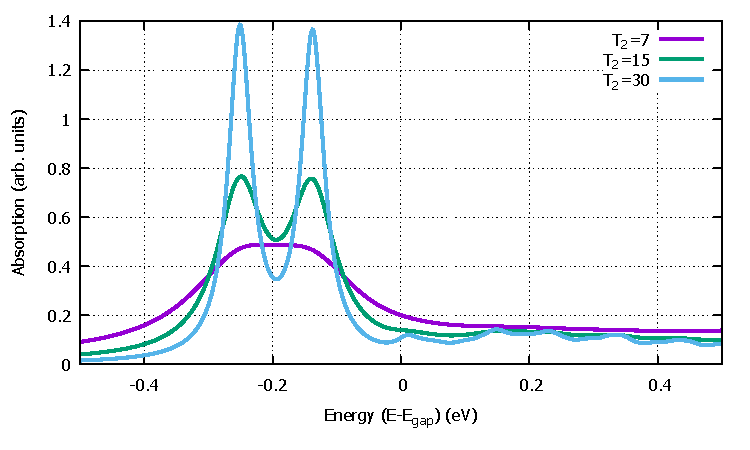
\includegraphics[width=0.75\linewidth]{images/varyT2.pdf}
		\caption[Absorption Spectrum with difference $T_2$]{Absorption Spectrum with difference $T_2$}
		\label{Vary T2}
	\end{center}
\end{figure}\null
\begin{figure}
	\begin{center}
		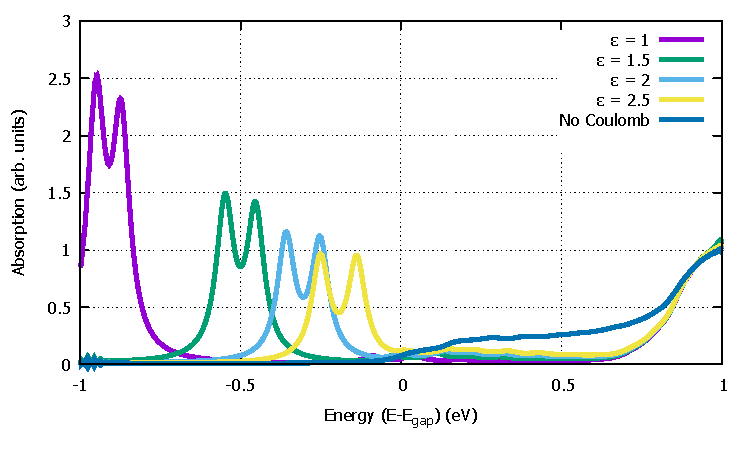
\includegraphics[width=0.75\linewidth]{images/varyepsilon.pdf}
		\caption[Absorption Spectrum with difference dielectric $\varepsilon$ and without Coulomb interaction]{Absorption Spectrum with difference dielectric $\varepsilon$ and without Coulomb interaction}
		\label{Vary e}
	\end{center}
\end{figure}\null
\quad This model is effective and has advantages for calculation over BZ, but it also has disadvantages and requires denser k-grids for results to converge (as shown in Fig. \ref{Vary nk}) compared to DFT models or parabola approximation models. The bare Coulomb interaction works well in calculating the linear absorption spectrum, but for a more realistic case, the shield Coulomb interaction must be taken into account\cite{erben_excitation-induced_2018,erben_optical_2022}, especially when we want to go beyond the small excitation limit. It's worth noting that the parameter $T_2$ is proved to be a good approximation without requiring further techniques in showing two main exciton peaks and predicting other smaller peaks. However, for a more realistic representation, the $T_2$ approximation can also be expanded in terms of electron-electron and electron-phonon scattering terms, which would provide a more comprehensive analysis of the system under consideration. Additionally, it is crucial to consider the implications of these findings in the context of practical applications and the broader theoretical framework.
\begin{figure}
	\begin{center}
		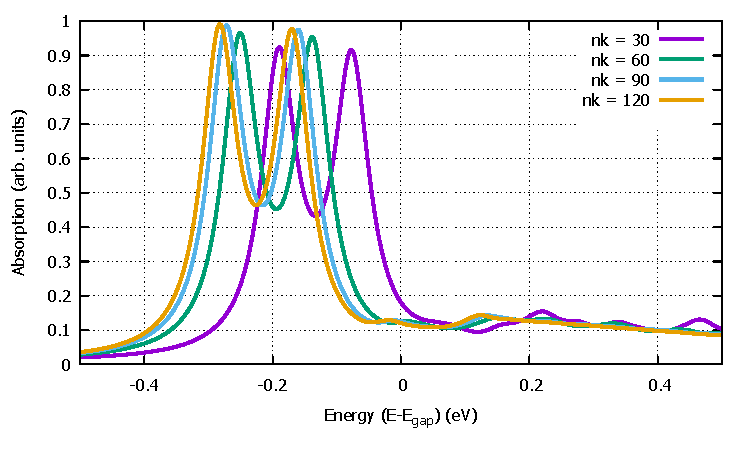
\includegraphics[width=0.75\linewidth]{images/varynk.pdf}
		\caption[Absorption Spectrum with difference number of k-points]{Absorption Spectrum with difference number of k-points}
		\label{Vary nk}
	\end{center}
\end{figure}\null
\newpage
\section{Conclusion and Further Research}
\quad In our research, we have calculated the linear absorption of monolayer $\mathrm{MoS}_2$ using a tight-binding three-band model with spin-orbit coupling through semiconductor Bloch equations in Hartree-Fock approximation. We have varied three parameters to analyze their relation with the absorption spectrum and found that the results align with other calculations, indicating a significant binding energy up to two magnitude in comparison with other bulk semiconductors.\\\null
\quad We have encountered some limitations, like the time-consuming process of enhancing the k-grid for better convergence and the discrepancy in the bandgap position as compared to experimental data. We also have observed that the bare Coulomb interaction might not be adequate for an accurate depiction and should be fine-tuned for better outcomes.\\\null
\quad For further researches, we can utilize this three-band tight-binding model to calculate other optoelectronic phenomena affected by excitons, such as high harmonic generation (HHG), high-order sideband generation (HSG), and photovoltaic current. When calculating the photovoltaic effect, it's important to consider the influence of Coulomb interactions. Without the consideration of Coulomb interactions, only the shift current is apparent, as we've calculated the current tensors as per Ref. \cite{vo_calculation_2024}. However, once we include the Coulomb interaction, the ballistic current becomes significant, and the shift tensor current is also affected. It's crucial to account for Coulomb interactions to obtain a realistic picture of the photovoltaic effect.

\newpage
\begin{appendices}
\begin{comment}
	\section{Electromagnetic Field - Charge Interaction Hamiltonian}
	\label{Electromagnetic Field - Charge Interaction Hamiltonian}
	\quad From classical Electromagnetic Interaction, we derive the Interaction Hamiltonian between an electric charge and a classical/semi-classical electromagnetic field. The Coulomb's force and Lorentz's force for an electric charge in an electromagnetic field have the following form:
	\begin{equation}
		\vec{F} = q (\vec{E} + \vec{v} \times \vec{B}).
	\end{equation}
	\quad From Euler-Largrange equation, we have
	\begin{equation}
		\label{C-L force}
		\vec{F} = - \vec{\nabla} U + \dv{ }{t} \bigg(\pdv{U}{\vec{v}}\bigg) ,
	\end{equation}
	\quad To satisfied (\ref{C-L force}), $U$ must be
	\begin{equation}
		U = q(\phi- \vec{v}.\vec{A}).
	\end{equation}
	\quad From it, we can construct the Largrangian of the Interaction between the electric charge and classical Electromagnetic field
	\begin{equation}
		L = T - U = \frac{1}{2}m \vec{v}^2 + q\vec{v}.\vec{A} -q\phi.
	\end{equation}
	\quad Canonical momentum for the charge is
	\begin{equation}
		\label{cannonical momentum}
		\vec{p} = \pdv{L}{\vec{v}} = m\vec{v} + q\vec{A}.
	\end{equation}
	\quad From that, we can construct classical Hamiltonian for electric charge in electromagnetic field
	\begin{equation}
		\label{classical H}
		H = \vec{p}.\vec{v} - L = \frac{1}{2m}\big(\vec{p} - q \vec{A}\big)^2 + q\phi.
	\end{equation}
	\quad To quantization Hamiltonian, we change the classical position and canonical momentum to position and canonical momentum operators, respectively
	$$\vec{p}\longrightarrow \hat{p}, \quad \vec{r}\longrightarrow \hat{r},$$ \null
	\quad include this into (\ref{classical H}) to get Hamiltonian operator:
	\begin{equation}
		\label{H operator}
		\hat{H} = \frac{1}{2m}\big(\hat{p} - q \vec{A}\big)^2 + q\phi
	\end{equation}
	\quad To confirm the Gauge variant of Schrödinger equation, we can start from it
	\begin{equation}
		\label{Schro}
		i \hbar \pdv{}{t}\psi = \hat{H}\psi = \bigg[\frac{1}{2m}\big(\hat{p} - q \vec{A}\big)^2 + q\phi\bigg] \psi.
	\end{equation}
	\quad Doing Gauge transform for the electromagnetic field and phase transform for the wave function
	$$\vec{A} \longrightarrow \vec{A} - \vec{\nabla} \chi,\quad \phi \longrightarrow \phi + \pdv{\chi}{t},\quad \psi \longrightarrow e^{-i\frac{q}{\hbar}\chi} \psi,$$
	\null \quad include it into (\ref{Schro}) to get
	\begin{equation*}
		i \hbar \pdv{}{t}e^{-i\frac{q}{\hbar}\chi} \psi  = \bigg[\frac{1}{2m}\big(\hat{p} - q (\vec{A} - \vec{\nabla} \chi)\big)^2 + q(\phi + \pdv{\chi}{t})\bigg] e^{-i\frac{q}{\hbar}\chi} \psi.
	\end{equation*}
	
	\newpage
\end{comment}
\section{Coulomb matrix elements}
\label{V ee derivation}
\begin{comment}
	\quad In this section, we will derive Hamiltonian for charge system in second quantization. Starting from Hamiltonian
	\begin{equation}
		H = \sum_{\textbf{k}} \varepsilon_\textbf{k} c_\textbf{k}^\dg c_\textbf{k} + \frac{1}{2} \sum_{\textbf{k}, \textbf{k}', \textbf{q}} \sum_{\alpha \beta \gamma \delta} W^{\alpha \beta \gamma \delta}_{\textbf{k},\textbf{k'},\textbf{q}} c_{\alpha, \textbf{k}+\textbf{q}}^\dg c_{\beta, \textbf{k}' - \textbf{q}}^\dg c_{\gamma, \textbf{k}}c_{\delta, \textbf{k'}}
	\end{equation}
\end{comment}
\quad The Coulomb matrix elements is
\begin{equation*}
	W^{\alpha \beta \gamma \delta}_{\textbf{k}, \textbf{k}', \textbf{q}} = \bra{\psi_{\alpha \textbf{k + q}} \psi_{\beta \textbf{k}' - \textbf{q}}} V_{e-e} \ket{\psi_{\gamma \textbf{k}'} \psi_{\delta \textbf{k}}}
	= 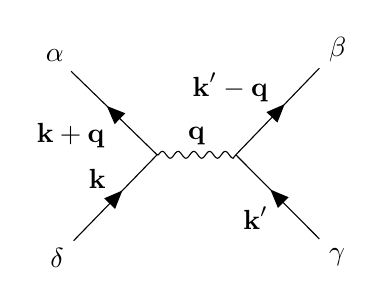
\begin{tikzpicture}
		\begin{feynman}
			% Define vertices
			\vertex (a);
			\vertex[below left= 1.5 cm of a] (i1) {\(\delta\)};
			\vertex[above left =  1.5 cm of a] (f1) {\(\alpha\)};
			\vertex[right = 1 cm of a] (b);
			\vertex[below right = 1.5 cm of b] (i2) {\(\gamma\)};
			\vertex[above right= 1.5 cm of b] (f2) {\(\beta\)};
			
			% Draw fermion lines
			\diagram*[horizontal'= (a) to (b)] {
				(i1) -- [fermion, edge label=$\textbf{k}$] (a) -- [fermion, edge label=$ \textbf{k} + \textbf{q}$] (f1),
				(i2) -- [fermion, edge label=$\textbf{k}'$] (b) -- [fermion, edge label={$\textbf{k}'- \textbf{q}$}] (f2),
				(a) -- [photon, edge label=$\textbf{q}$] (b),
			};
		\end{feynman}
	\end{tikzpicture}
\end{equation*}
\begin{equation}
\label{V element}
 = \int \frac{d^3 r}{V} \int \frac{d^3 r'}{V} e^{-i \textbf{q}(\textbf{r}-\textbf{r}')} u^*_{\alpha\textbf{k}+\textbf{q}}(\textbf{r})u^*_{\beta\textbf{k}-\textbf{q}}(\textbf{r}') V_{e-e}(\textbf{r}-\textbf{r}') u_{\gamma \textbf{k}'}(\textbf{r}')u_{\delta \textbf{k}}(\textbf{r}),
 \end{equation}
\quad with
\begin{equation}
	V_{e-e}(\textbf{r}) = \frac{e^2}{4\pi \varepsilon \varepsilon_0}\frac{1} {|\textbf{r}|},
\end{equation}
\quad we expand it using Fourier transform
\begin{align}
	V_{e-e} (\textbf{q}) &= \int \frac{d^3 \textbf{r}}{V} V_{e-e}(\textbf{r}) e^{-i \textbf{q}.\textbf{r}} = \frac{e^2}{4\pi \varepsilon \varepsilon_0 V} \int d^3 \textbf{r} \frac{1}{|\textbf{r}|} e^{-i\textbf{q}.\textbf{r}} \nonumber\\
	&= \frac{e^2}{4\pi \varepsilon \varepsilon_0 V} \int_0^{\infty} \int_{0}^{2\pi} \int_{-\pi}^{\pi}\frac{1}{r} r^2 e^{-i qr\cos(\theta)} dr d\varphi \cos{( \theta )} d\theta\nonumber \\
	&= \frac{e^2}{2 \varepsilon \varepsilon_0 V}\int_0^{\infty} \int_{-1}^{1} r dr d\cos\theta e^{i q r cos\theta} =-\frac{i}{q} \frac{e^2}{2 \varepsilon \varepsilon_0 V} \int_{0}^{\infty} dr (e^{iqr} - e^{-iqr})\nonumber \\
	& = -\frac{i}{q} \frac{e^2}{2 \varepsilon \varepsilon_0 V} \lim_{\gamma \to 0}\int_{0}^{\infty} dr (e^{iqr} - e^{-iqr}) e^{- \gamma r} \nonumber \\ \label{Coulomb q}&= \frac{e^2}{2\varepsilon \varepsilon_0
	 V} \lim_{\gamma \to 0}   \bigg(\int_0^{\infty}\frac{e^{(iq-\gamma)r}}{iq - \gamma} dr - \int_0^{\infty} \frac{e^{-(i q+\gamma)r}}{iq + \gamma} dr\bigg) = \frac{e^2}{\varepsilon \varepsilon_0 V} \frac{1}{q^2}.
\end{align}
Include (\ref{Coulomb q}) into (\ref{V element}) through reverse Fourier transform
\begin{align}
	\label{reverse Fourier}
	V_{e-e} (\textbf{r}) &= \sum_{\textbf{q}}V_{e-e}(\textbf{q}) e^{i\textbf{q}\textbf{r}} = \sum_{\textbf{q}_{||},\textbf{q}_{\perp}} \frac{e^2}{\varepsilon \varepsilon_0 V} \frac{1}{\textbf{q}_{||}^2 +q_{\perp}^2} e^{i\textbf{q}_{||}\textbf{r}_{||}} e^{iq_{\perp} r_{\perp}} \nonumber \\
	&= \sum_{\textbf{q}_{||}}\frac{1}{2\pi/L_z}\frac{e^2}{\varepsilon \varepsilon_0 V} e^{i\textbf{q}_{||} \textbf{r}_{||}} \int dq_{\perp}\frac{e^{iq_{\perp}r_{\perp}}}{\textbf{q}_{||}^2 +q_{\perp}^2}, \\ \bullet
	\int_{-\infty}^{\infty} dx \frac{e^{iax}}{a^2 +x^2} &= \oint dz \frac{e^{iaz}}{(z+ia)(z - ia)} = 2\pi i\Res_{z=ia}\bigg[\frac{e^{iax}}{(z+ia)(z - ia)}\bigg] \nonumber\\
	&= 2\pi i \lim_{z \to ia}\frac{e^{iax}}{(z+ia)(z - ia)} (z-ia) = 2\pi i \frac{e^{-ax}}{2ia} = \frac{\pi e^{-ax}}{a} \quad (a > 0)\\ \label{Revere Fourier}
	 \Rightarrow \quad 
	(\ref{reverse Fourier}) &= \sum_{\textbf{q}_{||}} \frac{e^2}{2 \varepsilon \varepsilon_0 V_{||} }e^{i\textbf{q}_{||} \textbf{r}_{||}} \frac{e^{-|\textbf{q}_{||}||\textbf{r}_{\perp}|}}{|\textbf{q}_{||}|} = \sum_{\textbf{q}_{||}}V^{2D}_{||}(\textbf{q}_{||}, \textbf{r}_\perp) e^{i\textbf{q}_{||}\textbf{r}{||}}
\end{align}
\begin{equation}
	\label{V Coulomb 2d}
	\therefore \quad V^{2D}_{||}(\textbf{q}_{||}, z) = \frac{e^2}{2 \varepsilon \varepsilon_0 V_{||} }\frac{e^{- |\textbf{q}_{||}| |z|}}{|\textbf{q}_{||}|}.
\end{equation}
\quad Include (\ref{V Coulomb 2d}) back into (\ref{V element}) through (\ref{Revere Fourier}) for 2D-case
\begin{align}
	&W^{\alpha\beta\gamma \delta}_{\textbf{k},\textbf{k'},\textbf{q}}= \int \int d\textbf{r}_1 d\textbf{r}_2 u_{\textbf{k}_{||}+\textbf{q}_{||}}^{\alpha\dg}(\textbf{r}_1) u ^{\beta \dg}_{\textbf{k}'_{||}-\textbf{q}_{||}}(\textbf{r}_2) V^{3D}(\textbf{r}_2 - \textbf{r}_1) e^{i\textbf{q}_{||}(\textbf{r}_2 - \textbf{r}_1)} u^\gamma_{\textbf{k}'_{||}}(\textbf{r}_2) u^{\delta}_{\textbf{k}_{||}}(\textbf{r}_1)\\
	&=\frac{e^2}{2 \varepsilon \varepsilon_0 V_{||}}\sum_{\textbf{q}'_{||}}\int \int d\textbf{r}_1 d\textbf{r}_2 u_{\textbf{k}_{||}+\textbf{q}_{||}}^{\alpha\dg}(\textbf{r}_1) u ^{\beta \dg}_{\textbf{k}'_{||}-\textbf{q}_{||}}(\textbf{r}_2)e^{i\textbf{q}'_{||} (\textbf{r}_{2||} - \textbf{r}_{1||})}\frac{e^{-|\textbf{q}'_{||}||z_2-z_1|}}{|\textbf{q}'_{||}|} e^{i\textbf{q}_{||}(\textbf{r}_2 - \textbf{r}_1)} u^\gamma_{\textbf{k}'_{||}}(\textbf{r}_2) u^{\delta}_{\textbf{k}_{||}}(\textbf{r}_1)\nonumber,
\end{align}
\quad We take the limit $z_1, z_2 \to 0$, therefore the $W^{\alpha\beta\gamma \delta}_{\textbf{k},\textbf{k'},\textbf{q}}$ take the form:
\begin{equation}
	W^{\alpha\beta\gamma \delta}_{\textbf{k},\textbf{k'},\textbf{q}} = \frac{e^2}{2\varepsilon \varepsilon_0 V_{||}} \sum_{\textbf{q}} \frac{1}{|\textbf{q}|} \braket{u_{\textbf{k}+\textbf{q}}^{\alpha}}{u^{\delta}_{\textbf{k}}} \braket{u ^{\beta}_{\textbf{k}'-\textbf{q}}}{u^\gamma_{\textbf{k}'}}
\end{equation}
\newpage
\section{Equation of Motion}
\label{Motion Equation}
\quad We consider Hamiltonian (\ref{H with Coulomb in second}), using Heisenberg motion equation part by part with creation and annihilation operator satisfies (\ref{fermion comm}):
\begin{align}
	\comm{H^{0}_{1e}}{c^\dg_{\alpha \textbf{k}} c_{\beta \textbf{k}}} &= \sum_{\textbf{k}' \lambda} \varepsilon_{\lambda,\textbf{k}'} \comm{c^\dg_{\lambda \textbf{k}'} c_{\lambda \textbf{k}'}}{c^\dg_{\alpha \textbf{k}} c_{\beta \textbf{k}}} \nonumber \\
	&= \sum_{\textbf{k}' \lambda} \varepsilon_{\lambda,\textbf{k}'} (c^\dg_{\lambda \textbf{k}'} c_{\lambda \textbf{k}'}c^\dg_{\alpha \textbf{k}} c_{\beta \textbf{k}} - c^\dg_{\alpha \textbf{k}} c_{\beta \textbf{k}}c^\dg_{\lambda \textbf{k}'} c_{\lambda \textbf{k}'})\nonumber \\
	& = \sum_{\textbf{k}\lambda'} \varepsilon_{\lambda,\textbf{k}}(c^\dg_{\lambda \textbf{k}'} \delta_{\lambda \alpha}\delta_{\textbf{k}\textbf{k}'} c_{\beta \textbf{k}} 
	- c^\dg_{\lambda \textbf{k}'}c^\dg_{\alpha \textbf{k}} c_{\lambda \textbf{k}'} c_{\beta \textbf{k}} 
	- c^\dg_{\alpha \textbf{k}} \delta_{\beta\lambda}\delta_{\textbf{k}\textbf{k}'} c_{\lambda \textbf{k}'} 
	+ c^\dg_{\alpha \textbf{k}}c^\dg_{\lambda \textbf{k}'} c_{\beta \textbf{k}} c_{\lambda \textbf{k}'}) \nonumber\\
	&= \sum_{\textbf{k}\lambda'} \varepsilon_{\lambda,\textbf{k}}(c^\dg_{\lambda \textbf{k}'} \delta_{\lambda \alpha}\delta_{\textbf{k}\textbf{k}'} c_{\beta \textbf{k}} 
	- \cancel{c^\dg_{\alpha \textbf{k}}c^\dg_{\lambda \textbf{k}'} c_{\beta \textbf{k}} c_{\lambda \textbf{k}'} }
	- c^\dg_{\alpha \textbf{k}} \delta_{\beta\lambda}\delta_{\textbf{k}\textbf{k}'} c_{\lambda \textbf{k}'} 
	+ \cancel{c^\dg_{\alpha \textbf{k}}c^\dg_{\lambda \textbf{k}'} c_{\beta \textbf{k}} c_{\lambda \textbf{k}'}})\nonumber\\\label{Energy commu}
	&= (\varepsilon_\alpha(\textbf{k}) - \varepsilon_{\beta}\textbf{(k)})c^\dg_{\alpha\textbf{k}} c_{\beta\textbf{k}}
\end{align}
\begin{align}
	\comm{H^{e-L}}{c^\dg_{\alpha \textbf{k}} c_{\beta \textbf{k}}} &= \sum_{\lambda\lambda' \textbf{k}'}\textbf{p}_{\lambda\lambda'}(\textbf{k}')\comm{c^\dg_{\lambda\textbf{k}'}c_{\lambda'\textbf{k}'}}{c_{\alpha \textbf{k}}^\dg c_{\beta \textbf{k}}} + \sum_{\lambda\textbf{k}'} \bigg(\hbar\textbf{k}'+\frac{e^2 A^2}{2m}\bigg) \cancel{\comm{c^\dg_{\lambda\textbf{k}'}c_{\lambda \textbf{k}'}}{c_{\alpha\textbf{k}}^\dg c_{\beta \textbf{k}}}}\nonumber \\
	&=\sum_{\lambda\lambda' \textbf{k}'}\textbf{p}_{\lambda\lambda'}(\textbf{k}')(c^\dg_{\lambda\textbf{k}'}c_{\lambda'\textbf{k}'}c_{\alpha \textbf{k}}^\dg c_{\beta \textbf{k}} - c_{\alpha \textbf{k}}^\dg c_{\beta \textbf{k}}c^\dg_{\lambda\textbf{k}'}c_{\lambda'\textbf{k}'})\nonumber  \nonumber\\
	&=\sum_{\lambda\lambda' \textbf{k}'}\textbf{p}_{\lambda\lambda'}(\textbf{k}')(c^\dg_{\lambda\textbf{k}'}\delta_{\lambda'\alpha} \delta_{\textbf{k}\textbf{k}'}c_{\beta \textbf{k}} -c^\dg_{\lambda\textbf{k}'}c_{\alpha \textbf{k}}^\dg c_{\lambda'\textbf{k}'}c_{\beta \textbf{k}}
	- c_{\alpha \textbf{k}}^\dg \delta_{\beta \lambda}\delta_{\textbf{k}\textbf{k}'} c_{\lambda'\textbf{k}'}
	+ c_{\alpha \textbf{k}}^\dg c^\dg_{\lambda\textbf{k}'} c_{\beta \textbf{k}}c_{\lambda'\textbf{k}'}
	)\nonumber\\
	&= \sum_{\lambda\lambda' \textbf{k}'}\textbf{p}_{\lambda\lambda'}(\textbf{k}')(c^\dg_{\lambda\textbf{k}'}\delta_{\lambda'\alpha} \delta_{\textbf{k}\textbf{k}'}c_{\beta \textbf{k}} -\cancel{c^\dg_{\lambda\textbf{k}'}c_{\alpha \textbf{k}}^\dg c_{\lambda'\textbf{k}'}c_{\beta \textbf{k}}}
	- c_{\alpha \textbf{k}}^\dg \delta_{\beta \lambda}\delta_{\textbf{k}\textbf{k}'} c_{\lambda'\textbf{k}'}
	+ \cancel{c_{\alpha \textbf{k}}^\dg c^\dg_{\lambda\textbf{k}'} c_{\beta \textbf{k}}c_{\lambda'\textbf{k}'}}
	)\nonumber\\ \label{Interaction commu}
	&= \sum_{\lambda}(\textbf{p}_{\lambda \alpha}(\textbf{k}) c^\dg_{\lambda \textbf{k}} c_{\beta \textbf{k}} - \textbf{P}_{\beta\lambda'}(\textbf{k}) c^\dg_{\alpha\textbf{k}}c_{\lambda'\textbf{k}})
\end{align}
\begin{align}
	\comm{H^{Coulomb}}{c^\dg_{\lambda \textbf{k}''} c_{\lambda' \textbf{k}''}} &= \sum_{\textbf{k}, \textbf{k}', \textbf{q}} \sum_{\alpha \beta \gamma \delta} W^{\alpha \beta \gamma \delta}_{\textbf{k},\textbf{k'},\textbf{q}}\comm{ c_{\alpha, \textbf{k}+\textbf{q}}^\dg c_{\beta, \textbf{k}' - \textbf{q}}^\dg c_{\gamma, \textbf{k}}c_{\delta, \textbf{k'}}}{c^\dg_{\lambda \textbf{k}''} c_{\lambda' \textbf{k}''}} \nonumber\\
	&= \sum_{\textbf{k}, \textbf{k}', \textbf{q}} \sum_{\alpha \beta \gamma \delta} W^{\alpha \beta \gamma \delta}_{\textbf{k},\textbf{k'},\textbf{q}}( c_{\alpha, \textbf{k}+\textbf{q}}^\dg c_{\beta, \textbf{k}' - \textbf{q}}^\dg c_{\gamma, \textbf{k}}c_{\delta, \textbf{k'}}c^\dg_{\lambda \textbf{k}''} c_{\lambda' \textbf{k}''} 
	-  c^\dg_{\lambda \textbf{k}''} c_{\lambda' \textbf{k}''}c_{\alpha, \textbf{k}+\textbf{q}}^\dg c_{\beta, \textbf{k}' - \textbf{q}}^\dg c_{\gamma, \textbf{k}}c_{\delta, \textbf{k'}}) \nonumber \\
	%
	%
\bullet	 \quad c_{\alpha, \textbf{k}+\textbf{q}}^\dg c_{\beta, \textbf{k}' - \textbf{q}}^\dg &c_{\gamma, \textbf{k}}c_{\delta, \textbf{k'}}c^\dg_{\lambda \textbf{k}''} c_{\lambda' \textbf{k}''} = c_{\alpha, \textbf{k}+\textbf{q}}^\dg c_{\beta, \textbf{k}' - \textbf{q}}^\dg c_{\gamma, \textbf{k}}\delta_{\lambda,\delta} \delta_{\textbf{k}',\textbf{k}''} c_{\lambda' \textbf{k}''} - c_{\alpha, \textbf{k}+\textbf{q}}^\dg c_{\beta, \textbf{k}' - \textbf{q}}^\dg c_{\gamma, \textbf{k}} c^\dg_{\lambda \textbf{k}''}c_{\delta, \textbf{k'}} c_{\lambda' \textbf{k}''} \nonumber\\
%
%
= c_{\alpha, \textbf{k}+\textbf{q}}^\dg c_{\beta, \textbf{k}' - \textbf{q}}^\dg c_{\gamma, \textbf{k}}&\delta_{\lambda,\delta} \delta_{\textbf{k}',\textbf{k}''} c_{\lambda' \textbf{k}''} - c_{\alpha, \textbf{k}+\textbf{q}}^\dg c_{\beta, \textbf{k}' - \textbf{q}}^\dg \delta_{\lambda \gamma} \delta_{\textbf{k}\textbf{k}''}c_{\delta, \textbf{k'}} c_{\lambda' \textbf{k}''} 
+ \cancel{c_{\alpha, \textbf{k}+\textbf{q}}^\dg c_{\beta, \textbf{k}' - \textbf{q}}^\dg c^\dg_{\lambda \textbf{k}''}c_{\gamma, \textbf{k}} c_{\delta, \textbf{k'}} c_{\lambda' \textbf{k}''}}\nonumber \\
%
%
\bullet	 \quad c^\dg_{\lambda \textbf{k}''} c_{\lambda' \textbf{k}''} c_{\alpha, \textbf{k}+\textbf{q}}^\dg &c_{\beta, \textbf{k}' - \textbf{q}}^\dg c_{\gamma, \textbf{k}}c_{\delta, \textbf{k'}} = c^\dg_{\lambda \textbf{k}''} \delta_{\lambda',\alpha} \delta_{\textbf{k}'',\textbf{k}+q} c_{\beta, \textbf{k}' - \textbf{q}}^\dg c_{\gamma, \textbf{k}}c_{\delta, \textbf{k'}} - c^\dg_{\lambda \textbf{k}''}  c_{\alpha, \textbf{k}+\textbf{q}}^\dg c_{\lambda' \textbf{k}''} c_{\beta, \textbf{k}' - \textbf{q}}^\dg c_{\gamma, \textbf{k}}c_{\delta, \textbf{k'}} \nonumber\\
= c^\dg_{\lambda \textbf{k}''} \delta_{\lambda',\alpha} \delta_{\textbf{k}'',\textbf{k}+q} &c_{\beta, \textbf{k}' - \textbf{q}}^\dg c_{\gamma, \textbf{k}}c_{\delta, \textbf{k'}} - c^\dg_{\lambda \textbf{k}''}  c_{\alpha, \textbf{k}+\textbf{q}}^\dg \delta_{\lambda'\beta} \delta_{\textbf{k}'',\textbf{k}'-\textbf{q}} c_{\gamma, \textbf{k}}c_{\delta, \textbf{k'}}
+ \cancel{c^\dg_{\lambda \textbf{k}''}  c_{\alpha, \textbf{k}+\textbf{q}}^\dg c_{\beta, \textbf{k}' - \textbf{q}}^\dg c_{\lambda' \textbf{k}''}  c_{\gamma, \textbf{k}}c_{\delta, \textbf{k'}}} \nonumber\\
%
%
\comm{H^{Coulomb}}{c^\dg_{\lambda \textbf{k}''} c_{\lambda' \textbf{k}''}} &= \sum_{\textbf{k}, \textbf{k}', \textbf{q}} \sum_{\alpha \beta \gamma \delta} W^{\alpha \beta \gamma \delta}_{\textbf{k},\textbf{k'},\textbf{q}}(c_{\alpha, \textbf{k}+\textbf{q}}^\dg c_{\beta, \textbf{k}' - \textbf{q}}^\dg c_{\gamma, \textbf{k}}\delta_{\lambda,\delta} \delta_{\textbf{k}',\textbf{k}''} c_{\lambda' \textbf{k}''} - c_{\alpha, \textbf{k}+\textbf{q}}^\dg c_{\beta, \textbf{k}' - \textbf{q}}^\dg \delta_{\lambda \gamma} \delta_{\textbf{k}\textbf{k}''}c_{\delta, \textbf{k'}} c_{\lambda' \textbf{k}''}\nonumber \\
&- c^\dg_{\lambda \textbf{k}''} \delta_{\lambda',\alpha} \delta_{\textbf{k}'',\textbf{k}+\textbf{q}} c_{\beta, \textbf{k}' - \textbf{q}}^\dg c_{\gamma, \textbf{k}}c_{\delta, \textbf{k'}} + c^\dg_{\lambda \textbf{k}''}  c_{\alpha, \textbf{k}+\textbf{q}}^\dg \delta_{\lambda'\beta} \delta_{\textbf{k}'',\textbf{k}'-\textbf{q}} c_{\gamma, \textbf{k}}c_{\delta, \textbf{k'}})\nonumber
\end{align}
\begin{align}
	&= \sum_{\textbf{k}, \textbf{k}', \textbf{q}} \sum_{\alpha \beta \gamma \delta} W^{\alpha \beta \gamma \delta}_{\textbf{k},\textbf{k'},\textbf{q}}c_{\alpha, \textbf{k}+\textbf{q}}^\dg c_{\beta, \textbf{k}' - \textbf{q}}^\dg c_{\gamma, \textbf{k}}\delta_{\lambda,\delta} \delta_{\textbf{k}',\textbf{k}''} c_{\lambda' \textbf{k}''}- \sum_{\textbf{k}, \textbf{k}', \textbf{q}} \sum_{\alpha \beta \gamma \delta} W^{\alpha \beta \gamma \delta}_{\textbf{k},\textbf{k'},\textbf{q}}c_{\alpha, \textbf{k}+\textbf{q}}^\dg c_{\beta, \textbf{k}' - \textbf{q}}^\dg \delta_{\lambda \gamma} \delta_{\textbf{k}\textbf{k}''}c_{\delta, \textbf{k'}} c_{\lambda' \textbf{k}''}\nonumber \\
	%
	%
	&- \sum_{\textbf{k}, \textbf{k}', \textbf{q}} \sum_{\alpha \beta \gamma \delta} W^{\alpha \beta \gamma \delta}_{\textbf{k},\textbf{k'},\textbf{q}}c^\dg_{\lambda \textbf{k}''} \delta_{\lambda',\alpha} \delta_{\textbf{k}'',\textbf{k}+\textbf{q}} c_{\beta, \textbf{k}' - \textbf{q}}^\dg c_{\gamma, \textbf{k}}c_{\delta, \textbf{k'}} + \sum_{\textbf{k}, \textbf{k}', \textbf{q}} \sum_{\alpha \beta \gamma \delta} W^{\alpha \beta \gamma \delta}_{\textbf{k},\textbf{k'},\textbf{q}}c^\dg_{\lambda \textbf{k}''}  c_{\alpha, \textbf{k}+\textbf{q}}^\dg \delta_{\lambda'\beta} \delta_{\textbf{k}'',\textbf{k}'-\textbf{q}} c_{\gamma, \textbf{k}}c_{\delta, \textbf{k'}}\nonumber \\
	%
	%
	&= \sum_{\textbf{k}, \textbf{q}} \sum_{\alpha \beta \gamma} W^{\alpha \beta \gamma \lambda}_{\textbf{k},\textbf{k}'',\textbf{q}}c_{\alpha, \textbf{k}+\textbf{q}}^\dg c_{\beta, \textbf{k}'' - \textbf{q}}^\dg c_{\gamma, \textbf{k}} c_{\lambda' \textbf{k}''}-
	%
	\sum_{\textbf{k}', \textbf{q}} \sum_{\alpha \beta \delta} W^{\alpha \beta \lambda \delta}_{\textbf{k}'',\textbf{k'},\textbf{q}}c_{\alpha, \textbf{k}''+\textbf{q}}^\dg c_{\beta, \textbf{k}' - \textbf{q}}^\dg c_{\delta, \textbf{k'}} c_{\lambda' \textbf{k}''}\nonumber \\
	%
	%
	&- \sum_{ \textbf{k}', \textbf{q}} \sum_{ \beta \gamma \delta} W^{\lambda' \beta \gamma \delta}_{\textbf{k}''-\textbf{q},\textbf{k'},\textbf{q}}c^\dg_{\lambda \textbf{k}''} c_{\beta, \textbf{k}' - \textbf{q}}^\dg c_{\gamma, \textbf{k}'' - \textbf{q}}c_{\delta, \textbf{k'}} + \sum_{\textbf{k}, \textbf{q}} \sum_{\alpha \gamma \delta} W^{\alpha \lambda' \gamma \delta}_{\textbf{k},\textbf{k'},\textbf{q}}c^\dg_{\lambda \textbf{k}''}  c_{\alpha, \textbf{k}+\textbf{q}}^\dg c_{\gamma, \textbf{k}}c_{\delta, \textbf{k}''+\textbf{q}}\nonumber\\
	&= \sum_{\textbf{k}, \textbf{q}} \sum_{\alpha \beta \gamma} W^{\alpha \beta \gamma \lambda}_{\textbf{k},\textbf{k}'',\textbf{q}}c_{\alpha, \textbf{k}+\textbf{q}}^\dg c_{\beta, \textbf{k}'' - \textbf{q}}^\dg c_{\gamma, \textbf{k}} c_{\lambda' \textbf{k}''}-
	%
	\sum_{\textbf{k}', \textbf{q}} \sum_{\alpha \beta \delta} W^{\alpha \beta \lambda \delta}_{\textbf{k}'',\textbf{k'},\textbf{q}}c_{\alpha, \textbf{k}''+\textbf{q}}^\dg c_{\beta, \textbf{k}' - \textbf{q}}^\dg c_{\delta, \textbf{k'}} c_{\lambda' \textbf{k}''}\nonumber \\
	%
	%
	&- \sum_{ \textbf{k}', \textbf{q}} \sum_{ \beta \gamma \delta} W^{\lambda' \beta \gamma \delta}_{\textbf{k}''-\textbf{q},\textbf{k'},\textbf{q}}c^\dg_{\lambda \textbf{k}''} c_{\beta, \textbf{k}' - \textbf{q}}^\dg c_{\gamma, \textbf{k}'' - \textbf{q}}c_{\delta, \textbf{k'}} + \sum_{\textbf{k}, \textbf{q}} \sum_{\alpha \gamma \delta} W^{\alpha \lambda' \gamma \delta}_{\textbf{k},\textbf{k'},\textbf{q}}c^\dg_{\lambda \textbf{k}''}  c_{\alpha, \textbf{k}+\textbf{q}}^\dg c_{\gamma, \textbf{k}}c_{\delta, \textbf{k}''+\textbf{q}}\nonumber \\ \label{Coulomb Commu}
	%
	&= 2 \sum_{\textbf{k}'\textbf{q}} \bigg(\sum_{\alpha \beta \gamma} W^{\alpha\beta\gamma \lambda}_{\textbf{k}'',\textbf{k} ',\textbf{q}} c^\dg_{\alpha \textbf{k}''+\textbf{q}} c^\dg_{\beta \textbf{k}'-\textbf{q}} c_{\gamma \textbf{k}'} c_{\lambda' \textbf{k}''} + W^{\alpha \lambda' \gamma \delta}_{\textbf{k}',\textbf{k}''+\textbf{q}, \textbf{q}}c^\dg_{\lambda \textbf{k}''} c^\dg_{\alpha \textbf{k}'+\textbf{q}}c_{\gamma \textbf{k}''+\textbf{q}}c_{\delta\textbf{k}'}\bigg)
\end{align}
\quad Using approximation for the 4-operators into the form of multiplication of 2-operators (Hatree-Fock approximation):
\begin{align}
	\sum_{\textbf{k}'\textbf{q}}\ev{c^\dg_{\alpha \textbf{k}''+\textbf{q}} c^\dg_{\beta \textbf{k}'-\textbf{q}} c_{\gamma \textbf{k}'} c_{\lambda' \textbf{k}''}} &= 	-\sum_{\textbf{k}'\textbf{q}} \ev{c^\dg_{\alpha \textbf{k}''+\textbf{q}}c_{\gamma\textbf{k}'}}\ev{c_{\beta \textbf{k}'-\textbf{q}}^\dg c_{\lambda' \textbf{k}''}} \delta_{\textbf{k}'\textbf{k}''}\nonumber\\\label{first HF}
	&= - \sum_{\textbf{q}}\ev{c^\dg_{\alpha \textbf{k}''+\textbf{q}} c_{\gamma \textbf{k}''+\textbf{q}}}\ev{c^\dg_{\textbf{k}''}c_{\lambda'\textbf{k}''}}\\
	%
	%
	\sum_{\textbf{k}'\textbf{q}} \ev{c^\dg_{\lambda \textbf{k}''} c^\dg_{\alpha \textbf{k}'+\textbf{q}}c_{\gamma \textbf{k}''+\textbf{q}}c_{\delta\textbf{k}'}} &= \sum_{\textbf{k}'\textbf{q}}\ev{c_{\lambda\textbf{k}''}^\dg c_{\delta\textbf{k}'}}\ev{c^\dg_{\alpha \textbf{k}'+\textbf{q}} c_{\gamma \textbf{k}''+\textbf{q}}}\delta_{\textbf{k}',\textbf{k}''}\nonumber \\\label{second HF}
	&= \sum_{\textbf{q}}\ev{c_{\lambda\textbf{k}''}^\dg c_{\delta\textbf{k}''}}\ev{c^\dg_{\alpha \textbf{k}''+\textbf{q}} c_{\gamma \textbf{k}''+\textbf{q}}}
\end{align}
\quad Include HFA (\ref{first HF}) and (\ref{second HF}) into (\ref{Coulomb Commu}).
Take all the communication term (\ref{Energy commu}), (\ref{Interaction commu}) and (\ref{Coulomb Commu}) into (\ref{Heisenberg eq}) to get the SBE in HFA:
\begin{align}
	\dv{ }{t}\rho_{\lambda\lambda'}(\textbf{k}) = &- \frac{i}{\hbar} (\varepsilon_\lambda(\textbf{k}) - \varepsilon_{\lambda'} (\textbf{k}))\rho_{\lambda \lambda'} - \frac{ie}{\hbar m} \textbf{A}(t)\sum_{\mu}(\textbf{p}_{\lambda\mu}(\textbf{k})\rho_{\mu \lambda'}(\textbf{k}) - \rho_{\lambda\mu}(\textbf{k})\textbf{p}_{\mu \lambda'}(\textbf{k})) \nonumber \\
	&+ \frac{i}{\hbar}(\Omega_{\lambda \mu}(\textbf{k})\rho_{\mu \lambda'}(\textbf{k}) - \rho_{\lambda\mu}(\textbf{k}) \Omega_{\mu \lambda'} (\textbf{k}))
\end{align}
\section{Dipole Matrix Elements}
\label{Dipole Matrix Elements}
\quad Starting from position matrix element:
\begin{align}
\bra{\psi_{\lambda \textbf{k}}}\textbf{r}\ket{\psi_{\lambda'\textbf{k}'}} &= \int \frac{d^3 r}{V} u^*_{\lambda \textbf{k}}(\textbf{r}) e^{-i\textbf{k}.\textbf{r}} \textbf{r} u_{\lambda' \textbf{k}'}(\textbf{r}) e^{i\textbf{k}'.\textbf{r}'}\\
&= i \nabla_\textbf{k} \bigg(\int \frac{d^3 r}{V} e^{-i\textbf{k}.\textbf{r}}u^*_{\lambda \textbf{k}}(\textbf{r}) u_{\lambda' \textbf{k}'}(\textbf{r})e^{i\textbf{k}'.\textbf{r}}\bigg) - \int \frac{d^3 r}{V} i e^{-i\textbf{k}\textbf{r}}(\nabla_\textbf{k} u^*_{\lambda \textbf{k}}) u_{\lambda' \textbf{k}'} e^{i\textbf{k}'\textbf{r}}\nonumber\\
&= i \nabla_\textbf{k} \bigg(\frac{1}{N} \sum_{i}^N e^{i(\textbf{k}'-\textbf{k}).\textbf{R}_i}\int_{V_{cell}} \frac{d^3 r}{V_{cell}} e^{-i\textbf{k}.\textbf{r}}u^*_{\lambda \textbf{k}}(\textbf{r}) u_{\lambda' \textbf{k}'}(\textbf{r})e^{i\textbf{k}'.\textbf{r}}\bigg)\nonumber\\
&\quad  - i\frac{1}{N}\sum_{i}^N e^{i(\textbf{k}'-\textbf{k}).\textbf{R}_i} \int_{V_{cell}} \frac{d^3 r}{V_{cell}} e^{i(\textbf{k}'-\textbf{k}).\textbf{r}} (\nabla_\textbf{k} u^*_{\lambda \textbf{k}}) u_{\lambda' \textbf{k}'}.
\end{align}
\quad Again, using the long-wavelength approximation to have
\begin{equation}
	\label{r after LWA}
	\bra{\psi_{\lambda \textbf{k}}}\textbf{r}\ket{\psi_{\lambda'\textbf{k}'}} \approx i \nabla_{\textbf{k}} \delta_{\textbf{k},\textbf{k}'}\delta_{\lambda \lambda'} - i \delta_{\textbf{k},\textbf{k}'} \braket{\nabla_\textbf{k}u_{\lambda \textbf{k}}}{u_{\lambda'\textbf{k}'}},
\end{equation}
\quad Define the dielectric matrix elements:
\begin{equation}
	\xi_{\lambda\lambda'}(\textbf{k}) = - i \braket{\nabla_\textbf{k}u_{\lambda \textbf{k}}}{u_{\lambda'\textbf{k}'}},
\end{equation}
\quad Include this into (\ref{r after LWA}) to have
\begin{equation}
	\bra{\psi_{\lambda \textbf{k}}}\textbf{r}\ket{\psi_{\lambda'\textbf{k}'}} = \delta_{\textbf{k},\textbf{k}'}(i\delta_{\lambda \lambda'} \nabla_{\textbf{k}}  +  \xi_{\lambda\lambda'}(\textbf{k})),
\end{equation}
Using this relation along with (\ref{p after LWA}) and $\comm{H^0_{1e}}{\textbf{r}} = -i\frac{\hbar}{m}\textbf{p}$ for $\lambda \neq \lambda'$:
\begin{equation}
	\xi_{\lambda\lambda'}(\textbf{k}) = -\frac{i\hbar}{m}\frac{\textbf{p}_{\lambda\lambda'}(\textbf{k})}{\varepsilon_{\lambda}(\textbf{\textbf{k}}) - \varepsilon_{\lambda'}(\textbf{k})}
\end{equation}
\end{appendices}
\newpage
\bibliographystyle{unsrt}
\bibliography{library}
\end{document}